\documentclass{article}

% if you need to pass options to natbib, use, e.g.:
%     \PassOptionsToPackage{numbers, compress}{natbib}
% before loading neurips_2024


% ready for submission
% \usepackage{neurips_2024}
\usepackage[preprint]{neurips_2024}
\usepackage{natbib}
% \usepackage[backend=bibtex]{biblatex}
% \usepackage[backend=biber]{biblatex}


% to compile a preprint version, e.g., for submission to arXiv, add add the
% [preprint] option:
%     \usepackage[preprint]{neurips_2024}


% to compile a camera-ready version, add the [final] option, e.g.:
%     \usepackage[final]{neurips_2024}


% to avoid loading the natbib package, add option nonatbib:
%    \usepackage[nonatbib]{neurips_2024}
  


\usepackage[utf8]{inputenc} % allow utf-8 input
\usepackage[T1]{fontenc}    % use 8-bit T1 fonts
\usepackage{hyperref}       % hyperlinks
\usepackage{url}            % simple URL typesetting
\usepackage{booktabs}       % professional-quality tables
\usepackage{amsfonts}       % blackboard math symbols
\usepackage{nicefrac}       % compact symbols for 1/2, etc.
\usepackage{microtype}      % microtypography
\usepackage{xcolor}         % colors
\usepackage{graphicx}
\usepackage{subcaption}
\usepackage{wrapfig}
\usepackage{todonotes}
\usepackage{array}
% \usepackage{amsmath}
\usepackage{booktabs}
\usepackage{amssymb}% http://ctan.org/pkg/amssymb
\usepackage{pifont}% http://ctan.org/pkg/pifont
\usepackage{tablefootnote}
\usepackage{tabularx}


\newcommand{\sysname}{AIBrix}
% \renewcommand{\cmark}{\ding{51}}%
\newcommand{\xmark}{\ding{55}}%
\renewcommand{\arraystretch}{1.3} 

% \addbibresource{references.bib} % Link the .bib file

\title{\sysname{}: Towards Scalable, Cost-Effective Large Language Model Inference Infrastructure}
%\title{\sysname{}: Towards Scalable, Cost-Effective AI Infrastructure for Generative AI}
 

% The \author macro works with any number of authors. There are two commands
% used to separate the names and addresses of multiple authors: \And and \AND.
%
% Using \And between authors leaves it to LaTeX to determine where to break the
% lines. Using \AND forces a line break at that point. So, if LaTeX puts 3 of 4
% authors names on the first line, and the last on the second line, try using
% \AND instead of \And before the third author name.

\author{%
  The AIBrix Team\\%\thanks{Use footnote for providing further information
    % about author (webpage, alternative address)---\emph{not} for acknowledging
    % funding agencies.} \\
  \texttt{maintainers@aibrix.ai} \\
}

% \author{%
%   David S.~Hippocampus\\%\thanks{Use footnote for providing further information
%     % about author (webpage, alternative address)---\emph{not} for acknowledging
%     % funding agencies.} \\
%   Department of Computer Science\\
%   Cranberry-Lemon University\\
%   Pittsburgh, PA 15213 \\
%   \texttt{hippo@cs.cranberry-lemon.edu} \\
%   % examples of more authors
%   % \And
%   % Coauthor \\
%   % Affiliation \\
%   % Address \\
%   % \texttt{email} \\
%   % \AND
%   % Coauthor \\
%   % Affiliation \\
%   % Address \\
%   % \texttt{email} \\
%   % \And
%   % Coauthor \\
%   % Affiliation \\
%   % Address \\
%   % \texttt{email} \\
%   % \And
%   % Coauthor \\
%   % Affiliation \\
%   % Address \\
%   % \texttt{email} \\
% }


\begin{document}


\maketitle


\begin{abstract}
  We introduce \sysname{}, a cloud-native, open-source framework designed to optimize and simplify large-scale LLM deployment in cloud environments.
  Unlike traditional cloud-native stacks, \sysname{} follows a co-design philosophy, ensuring every layer of the infrastructure is purpose-built for seamless integration with inference engines like vLLM.

  \sysname{} introduces several key innovations to reduce inference costs and enhance performance including high-density LoRA management for dynamic adapter scheduling, LLM-specific autoscalers, and prefix-aware, load-aware routing.
  To further improve efficiency, \sysname{} incorporates a distributed KV cache, boosting token reuse across nodes, leading to a 50\% increase in throughput and a 70\% reduction in inference latency.
  \sysname{} also supports unified AI runtime which streamlines model management while maintaining vendor-agnostic engine compatibility.

  
  For large-scale multi-node inference, \sysname{} employs hybrid orchestration—leveraging Kubernetes for coarse-grained scheduling and Ray for fine-grained execution—to balance efficiency and flexibility.
  Additionally, an SLO-driven GPU optimizer dynamically adjusts resource allocations, optimizing heterogeneous serving to maximize cost efficiency while maintaining service guarantees.
  Finally, \sysname{} enhances system reliability with AI accelerator diagnostic tools, enabling automated failure detection and mock-up testing to improve fault resilience.
  \sysname{} is available at \textcolor{red}{https://github.com/vllm-project/aibrix}.

\end{abstract}




\section{Introduction}


\begin{figure}[t]
\centering
\includegraphics[width=0.6\columnwidth]{figures/evaluation_desiderata_V5.pdf}
\vspace{-0.5cm}
\caption{\systemName is a platform for conducting realistic evaluations of code LLMs, collecting human preferences of coding models with real users, real tasks, and in realistic environments, aimed at addressing the limitations of existing evaluations.
}
\label{fig:motivation}
\end{figure}

\begin{figure*}[t]
\centering
\includegraphics[width=\textwidth]{figures/system_design_v2.png}
\caption{We introduce \systemName, a VSCode extension to collect human preferences of code directly in a developer's IDE. \systemName enables developers to use code completions from various models. The system comprises a) the interface in the user's IDE which presents paired completions to users (left), b) a sampling strategy that picks model pairs to reduce latency (right, top), and c) a prompting scheme that allows diverse LLMs to perform code completions with high fidelity.
Users can select between the top completion (green box) using \texttt{tab} or the bottom completion (blue box) using \texttt{shift+tab}.}
\label{fig:overview}
\end{figure*}

As model capabilities improve, large language models (LLMs) are increasingly integrated into user environments and workflows.
For example, software developers code with AI in integrated developer environments (IDEs)~\citep{peng2023impact}, doctors rely on notes generated through ambient listening~\citep{oberst2024science}, and lawyers consider case evidence identified by electronic discovery systems~\citep{yang2024beyond}.
Increasing deployment of models in productivity tools demands evaluation that more closely reflects real-world circumstances~\citep{hutchinson2022evaluation, saxon2024benchmarks, kapoor2024ai}.
While newer benchmarks and live platforms incorporate human feedback to capture real-world usage, they almost exclusively focus on evaluating LLMs in chat conversations~\citep{zheng2023judging,dubois2023alpacafarm,chiang2024chatbot, kirk2024the}.
Model evaluation must move beyond chat-based interactions and into specialized user environments.



 

In this work, we focus on evaluating LLM-based coding assistants. 
Despite the popularity of these tools---millions of developers use Github Copilot~\citep{Copilot}---existing
evaluations of the coding capabilities of new models exhibit multiple limitations (Figure~\ref{fig:motivation}, bottom).
Traditional ML benchmarks evaluate LLM capabilities by measuring how well a model can complete static, interview-style coding tasks~\citep{chen2021evaluating,austin2021program,jain2024livecodebench, white2024livebench} and lack \emph{real users}. 
User studies recruit real users to evaluate the effectiveness of LLMs as coding assistants, but are often limited to simple programming tasks as opposed to \emph{real tasks}~\citep{vaithilingam2022expectation,ross2023programmer, mozannar2024realhumaneval}.
Recent efforts to collect human feedback such as Chatbot Arena~\citep{chiang2024chatbot} are still removed from a \emph{realistic environment}, resulting in users and data that deviate from typical software development processes.
We introduce \systemName to address these limitations (Figure~\ref{fig:motivation}, top), and we describe our three main contributions below.


\textbf{We deploy \systemName in-the-wild to collect human preferences on code.} 
\systemName is a Visual Studio Code extension, collecting preferences directly in a developer's IDE within their actual workflow (Figure~\ref{fig:overview}).
\systemName provides developers with code completions, akin to the type of support provided by Github Copilot~\citep{Copilot}. 
Over the past 3 months, \systemName has served over~\completions suggestions from 10 state-of-the-art LLMs, 
gathering \sampleCount~votes from \userCount~users.
To collect user preferences,
\systemName presents a novel interface that shows users paired code completions from two different LLMs, which are determined based on a sampling strategy that aims to 
mitigate latency while preserving coverage across model comparisons.
Additionally, we devise a prompting scheme that allows a diverse set of models to perform code completions with high fidelity.
See Section~\ref{sec:system} and Section~\ref{sec:deployment} for details about system design and deployment respectively.



\textbf{We construct a leaderboard of user preferences and find notable differences from existing static benchmarks and human preference leaderboards.}
In general, we observe that smaller models seem to overperform in static benchmarks compared to our leaderboard, while performance among larger models is mixed (Section~\ref{sec:leaderboard_calculation}).
We attribute these differences to the fact that \systemName is exposed to users and tasks that differ drastically from code evaluations in the past. 
Our data spans 103 programming languages and 24 natural languages as well as a variety of real-world applications and code structures, while static benchmarks tend to focus on a specific programming and natural language and task (e.g. coding competition problems).
Additionally, while all of \systemName interactions contain code contexts and the majority involve infilling tasks, a much smaller fraction of Chatbot Arena's coding tasks contain code context, with infilling tasks appearing even more rarely. 
We analyze our data in depth in Section~\ref{subsec:comparison}.



\textbf{We derive new insights into user preferences of code by analyzing \systemName's diverse and distinct data distribution.}
We compare user preferences across different stratifications of input data (e.g., common versus rare languages) and observe which affect observed preferences most (Section~\ref{sec:analysis}).
For example, while user preferences stay relatively consistent across various programming languages, they differ drastically between different task categories (e.g. frontend/backend versus algorithm design).
We also observe variations in user preference due to different features related to code structure 
(e.g., context length and completion patterns).
We open-source \systemName and release a curated subset of code contexts.
Altogether, our results highlight the necessity of model evaluation in realistic and domain-specific settings.





\section{Bellman Error Centering}

Centering operator $\mathcal{C}$ for a variable $x(s)$ is defined as follows:
\begin{equation}
\mathcal{C}x(s)\dot{=} x(s)-\mathbb{E}[x(s)]=x(s)-\sum_s{d_{s}x(s)},
\end{equation} 
where $d_s$ is the probability of $s$.
In vector form,
\begin{equation}
\begin{split}
\mathcal{C}\bm{x} &= \bm{x}-\mathbb{E}[x]\bm{1}\\
&=\bm{x}-\bm{x}^{\top}\bm{d}\bm{1},
\end{split}
\end{equation} 
where $\bm{1}$ is an all-ones vector.
For any vector $\bm{x}$ and $\bm{y}$ with a same distribution $\bm{d}$,
we have
\begin{equation}
\begin{split}
\mathcal{C}(\bm{x}+\bm{y})&=(\bm{x}+\bm{y})-(\bm{x}+\bm{y})^{\top}\bm{d}\bm{1}\\
&=\bm{x}-\bm{x}^{\top}\bm{d}\bm{1}+\bm{y}-\bm{y}^{\top}\bm{d}\bm{1}\\
&=\mathcal{C}\bm{x}+\mathcal{C}\bm{y}.
\end{split}
\end{equation}
\subsection{Revisit Reward Centering}


The update (\ref{src3}) is an unbiased estimate of the average reward
with  appropriate learning rate $\beta_t$ conditions.
\begin{equation}
\bar{r}_{t}\approx \lim_{n\rightarrow\infty}\frac{1}{n}\sum_{t=1}^n\mathbb{E}_{\pi}[r_t].
\end{equation}
That is 
\begin{equation}
r_t-\bar{r}_{t}\approx r_t-\lim_{n\rightarrow\infty}\frac{1}{n}\sum_{t=1}^n\mathbb{E}_{\pi}[r_t]= \mathcal{C}r_t.
\end{equation}
Then, the simple reward centering can be rewrited as:
\begin{equation}
V_{t+1}(s_t)=V_{t}(s_t)+\alpha_t [\mathcal{C}r_{t+1}+\gamma V_{t}(s_{t+1})-V_t(s_t)].
\end{equation}
Therefore, the simple reward centering is, in a strict sense, reward centering.

By definition of $\bar{\delta}_t=\delta_t-\bar{r}_{t}$,
let rewrite the update rule of the value-based reward centering as follows:
\begin{equation}
V_{t+1}(s_t)=V_{t}(s_t)+\alpha_t \rho_t (\delta_t-\bar{r}_{t}),
\end{equation}
where $\bar{r}_{t}$ is updated as:
\begin{equation}
\bar{r}_{t+1}=\bar{r}_{t}+\beta_t \rho_t(\delta_t-\bar{r}_{t}).
\label{vrc3}
\end{equation}
The update (\ref{vrc3}) is an unbiased estimate of the TD error
with  appropriate learning rate $\beta_t$ conditions.
\begin{equation}
\bar{r}_{t}\approx \mathbb{E}_{\pi}[\delta_t].
\end{equation}
That is 
\begin{equation}
\delta_t-\bar{r}_{t}\approx \mathcal{C}\delta_t.
\end{equation}
Then, the value-based reward centering can be rewrited as:
\begin{equation}
V_{t+1}(s_t)=V_{t}(s_t)+\alpha_t \rho_t \mathcal{C}\delta_t.
\label{tdcentering}
\end{equation}
Therefore, the value-based reward centering is no more,
 in a strict sense, reward centering.
It is, in a strict sense, \textbf{Bellman error centering}.

It is worth noting that this understanding is crucial, 
as designing new algorithms requires leveraging this concept.


\subsection{On the Fixpoint Solution}

The update rule (\ref{tdcentering}) is a stochastic approximation
of the following update:
\begin{equation}
\begin{split}
V_{t+1}&=V_{t}+\alpha_t [\bm{\mathcal{T}}^{\pi}\bm{V}-\bm{V}-\mathbb{E}[\delta]\bm{1}]\\
&=V_{t}+\alpha_t [\bm{\mathcal{T}}^{\pi}\bm{V}-\bm{V}-(\bm{\mathcal{T}}^{\pi}\bm{V}-\bm{V})^{\top}\bm{d}_{\pi}\bm{1}]\\
&=V_{t}+\alpha_t [\mathcal{C}(\bm{\mathcal{T}}^{\pi}\bm{V}-\bm{V})].
\end{split}
\label{tdcenteringVector}
\end{equation}
If update rule (\ref{tdcenteringVector}) converges, it is expected that
$\mathcal{C}(\mathcal{T}^{\pi}V-V)=\bm{0}$.
That is 
\begin{equation}
    \begin{split}
    \mathcal{C}\bm{V} &= \mathcal{C}\bm{\mathcal{T}}^{\pi}\bm{V} \\
    &= \mathcal{C}(\bm{R}^{\pi} + \gamma \mathbb{P}^{\pi} \bm{V}) \\
    &= \mathcal{C}\bm{R}^{\pi} + \gamma \mathcal{C}\mathbb{P}^{\pi} \bm{V} \\
    &= \mathcal{C}\bm{R}^{\pi} + \gamma (\mathbb{P}^{\pi} \bm{V} - (\mathbb{P}^{\pi} \bm{V})^{\top} \bm{d_{\pi}} \bm{1}) \\
    &= \mathcal{C}\bm{R}^{\pi} + \gamma (\mathbb{P}^{\pi} \bm{V} - \bm{V}^{\top} (\mathbb{P}^{\pi})^{\top} \bm{d_{\pi}} \bm{1}) \\  % 修正双重上标
    &= \mathcal{C}\bm{R}^{\pi} + \gamma (\mathbb{P}^{\pi} \bm{V} - \bm{V}^{\top} \bm{d_{\pi}} \bm{1}) \\
    &= \mathcal{C}\bm{R}^{\pi} + \gamma (\mathbb{P}^{\pi} \bm{V} - \bm{V}^{\top} \bm{d_{\pi}} \mathbb{P}^{\pi} \bm{1}) \\
    &= \mathcal{C}\bm{R}^{\pi} + \gamma (\mathbb{P}^{\pi} \bm{V} - \mathbb{P}^{\pi} \bm{V}^{\top} \bm{d_{\pi}} \bm{1}) \\
    &= \mathcal{C}\bm{R}^{\pi} + \gamma \mathbb{P}^{\pi} (\bm{V} - \bm{V}^{\top} \bm{d_{\pi}} \bm{1}) \\
    &= \mathcal{C}\bm{R}^{\pi} + \gamma \mathbb{P}^{\pi} \mathcal{C}\bm{V} \\
    &\dot{=} \bm{\mathcal{T}}_c^{\pi} \mathcal{C}\bm{V},
    \end{split}
    \label{centeredfixpoint}
    \end{equation}
where we defined $\bm{\mathcal{T}}_c^{\pi}$ as a centered Bellman operator.
We call equation (\ref{centeredfixpoint}) as centered Bellman equation.
And it is \textbf{centered fixpoint}.

For linear value function approximation, let define
\begin{equation}
\mathcal{C}\bm{V}_{\bm{\theta}}=\bm{\Pi}\bm{\mathcal{T}}_c^{\pi}\mathcal{C}\bm{V}_{\bm{\theta}}.
\label{centeredTDfixpoint}
\end{equation}
We call equation (\ref{centeredTDfixpoint}) as \textbf{centered TD fixpoint}.

\subsection{On-policy and Off-policy Centered TD Algorithms
with Linear Value Function Approximation}
Given the above centered TD fixpoint,
 mean squared centered Bellman error (MSCBE), is proposed as follows:
\begin{align*}
    \label{argminMSBEC}
 &\arg \min_{{\bm{\theta}}}\text{MSCBE}({\bm{\theta}}) \\
 &= \arg \min_{{\bm{\theta}}} \|\bm{\mathcal{T}}_c^{\pi}\mathcal{C}\bm{V}_{\bm{{\bm{\theta}}}}-\mathcal{C}\bm{V}_{\bm{{\bm{\theta}}}}\|_{\bm{D}}^2\notag\\
 &=\arg \min_{{\bm{\theta}}} \|\bm{\mathcal{T}}^{\pi}\bm{V}_{\bm{{\bm{\theta}}}} - \bm{V}_{\bm{{\bm{\theta}}}}-(\bm{\mathcal{T}}^{\pi}\bm{V}_{\bm{{\bm{\theta}}}} - \bm{V}_{\bm{{\bm{\theta}}}})^{\top}\bm{d}\bm{1}\|_{\bm{D}}^2\notag\\
 &=\arg \min_{{\bm{\theta}},\omega} \| \bm{\mathcal{T}}^{\pi}\bm{V}_{\bm{{\bm{\theta}}}} - \bm{V}_{\bm{{\bm{\theta}}}}-\omega\bm{1} \|_{\bm{D}}^2\notag,
\end{align*}
where $\omega$ is is used to estimate the expected value of the Bellman error.
% where $\omega$ is used to estimate $\mathbb{E}[\delta]$, $\omega \doteq \mathbb{E}[\mathbb{E}[\delta_t|S_t]]=\mathbb{E}[\delta]$ and $\delta_t$ is the TD error as follows:
% \begin{equation}
% \delta_t = r_{t+1}+\gamma
% {\bm{\theta}}_t^{\top}\bm{{\bm{\phi}}}_{t+1}-{\bm{\theta}}_t^{\top}\bm{{\bm{\phi}}}_t.
% \label{delta}
% \end{equation}
% $\mathbb{E}[\delta_t|S_t]$ is the Bellman error, and $\mathbb{E}[\mathbb{E}[\delta_t|S_t]]$ represents the expected value of the Bellman error.
% If $X$ is a random variable and $\mathbb{E}[X]$ is its expected value, then $X-\mathbb{E}[X]$ represents the centered form of $X$. 
% Therefore, we refer to $\mathbb{E}[\delta_t|S_t]-\mathbb{E}[\mathbb{E}[\delta_t|S_t]]$ as Bellman error centering and 
% $\mathbb{E}[(\mathbb{E}[\delta_t|S_t]-\mathbb{E}[\mathbb{E}[\delta_t|S_t]])^2]$ represents the the mean squared centered Bellman error, namely MSCBE.
% The meaning of (\ref{argminMSBEC}) is to minimize the mean squared centered Bellman error.
%The derivation of CTD is as follows.

First, the parameter  $\omega$ is derived directly based on
stochastic gradient descent:
\begin{equation}
\omega_{t+1}= \omega_{t}+\beta_t(\delta_t-\omega_t).
\label{omega}
\end{equation}

Then, based on stochastic semi-gradient descent, the update of 
the parameter ${\bm{\theta}}$ is as follows:
\begin{equation}
{\bm{\theta}}_{t+1}=
{\bm{\theta}}_{t}+\alpha_t(\delta_t-\omega_t)\bm{{\bm{\phi}}}_t.
\label{theta}
\end{equation}

We call (\ref{omega}) and (\ref{theta}) the on-policy centered
TD (CTD) algorithm. The convergence analysis with be given in
the following section.

In off-policy learning, we can simply multiply by the importance sampling
 $\rho$.
\begin{equation}
    \omega_{t+1}=\omega_{t}+\beta_t\rho_t(\delta_t-\omega_t),
    \label{omegawithrho}
\end{equation}
\begin{equation}
    {\bm{\theta}}_{t+1}=
    {\bm{\theta}}_{t}+\alpha_t\rho_t(\delta_t-\omega_t)\bm{{\bm{\phi}}}_t.
    \label{thetawithrho}
\end{equation}

We call (\ref{omegawithrho}) and (\ref{thetawithrho}) the off-policy centered
TD (CTD) algorithm.

% By substituting $\delta_t$ into Equations (\ref{omegawithrho}) and (\ref{thetawithrho}), 
% we can see that Equations (\ref{thetawithrho}) and (\ref{omegawithrho}) are formally identical 
% to the linear expressions of Equations (\ref{rewardcentering1}) and (\ref{rewardcentering2}), respectively. However, the meanings 
% of the corresponding parameters are entirely different.
% ${\bm{\theta}}_t$ is for approximating the discounted value function.
% $\bar{r_t}$ is an estimate of the average reward, while $\omega_t$ 
% is an estimate of the expected value of the Bellman error.
% $\bar{\delta_t}$ is the TD error for value-based reward centering, 
% whereas $\delta_t$ is the traditional TD error.

% This study posits that the CTD is equivalent to value-based reward 
% centering. However, CTD can be unified under a single framework 
% through an objective function, MSCBE, which also lays the 
% foundation for proving the algorithm's convergence. 
% Section 4 demonstrates that the CTD algorithm guarantees 
% convergence in the on-policy setting.

\subsection{Off-policy Centered TDC Algorithm with Linear Value Function Approximation}
The convergence of the  off-policy centered TD algorithm
may not be guaranteed.

To deal with this problem, we propose another new objective function, 
called mean squared projected centered Bellman error (MSPCBE), 
and derive Centered TDC algorithm (CTDC).

% We first establish some relationships between
%  the vector-matrix quantities and the relevant statistical expectation terms:
% \begin{align*}
%     &\mathbb{E}[(\delta({\bm{\theta}})-\mathbb{E}[\delta({\bm{\theta}})]){\bm{\phi}}] \\
%     &= \sum_s \mu(s) {\bm{\phi}}(s) \big( R(s) + \gamma \sum_{s'} P_{ss'} V_{\bm{\theta}}(s') - V_{\bm{\theta}}(s)  \\
%     &\quad \quad-\sum_s \mu(s)(R(s) + \gamma \sum_{s'} P_{ss'} V_{\bm{\theta}}(s') - V_{\bm{\theta}}(s))\big)\\
%     &= \bm{\Phi}^\top \mathbf{D} (\bm{TV}_{\bm{{\bm{\theta}}}} - \bm{V}_{\bm{{\bm{\theta}}}}-\omega\bm{1}),
% \end{align*}
% where $\omega$ is the expected value of the Bellman error and $\bm{1}$ is all-ones vector.

The specific expression of the objective function 
MSPCBE is as follows:
\begin{align}
    \label{MSPBECwithomega}
    &\arg \min_{{\bm{\theta}}}\text{MSPCBE}({\bm{\theta}})\notag\\ 
    % &= \arg \min_{{\bm{\theta}}}\big(\mathbb{E}[(\delta({\bm{\theta}}) - \mathbb{E}[\delta({\bm{\theta}})]) \bm{{\bm{\phi}}}]^\top \notag\\
    % &\quad \quad \quad\mathbb{E}[\bm{{\bm{\phi}}} \bm{{\bm{\phi}}}^\top]^{-1} \mathbb{E}[(\delta({\bm{\theta}}) - \mathbb{E}[\delta({\bm{\theta}})]) \bm{{\bm{\phi}}}]\big) \notag\\
    % &=\arg \min_{{\bm{\theta}},\omega}\mathbb{E}[(\delta({\bm{\theta}})-\omega) \bm{\bm{{\bm{\phi}}}}]^{\top} \mathbb{E}[\bm{\bm{{\bm{\phi}}}} \bm{\bm{{\bm{\phi}}}}^{\top}]^{-1}\mathbb{E}[(\delta({\bm{\theta}}) -\omega)\bm{\bm{{\bm{\phi}}}}]\\
    % &= \big(\bm{\Phi}^\top \mathbf{D} (\bm{TV}_{\bm{{\bm{\theta}}}} - \bm{V}_{\bm{{\bm{\theta}}}}-\omega\bm{1})\big)^\top (\bm{\Phi}^\top \mathbf{D} \bm{\Phi})^{-1} \notag\\
    % & \quad \quad \quad \bm{\Phi}^\top \mathbf{D} (\bm{TV}_{\bm{{\bm{\theta}}}} - \bm{V}_{\bm{{\bm{\theta}}}}-\omega\bm{1}) \notag\\
    % &= (\bm{TV}_{\bm{{\bm{\theta}}}} - \bm{V}_{\bm{{\bm{\theta}}}}-\omega\bm{1})^\top \mathbf{D} \bm{\Phi} (\bm{\Phi}^\top \mathbf{D} \bm{\Phi})^{-1} \notag\\
    % &\quad \quad \quad \bm{\Phi}^\top \mathbf{D} (\bm{TV}_{\bm{{\bm{\theta}}}} - \bm{V}_{\bm{{\bm{\theta}}}}-\omega\bm{1})\notag\\
    % &= (\bm{TV}_{\bm{{\bm{\theta}}}} - \bm{V}_{\bm{{\bm{\theta}}}}-\omega\bm{1})^\top {\bm{\Pi}}^\top \mathbf{D} {\bm{\Pi}} (\bm{TV}_{\bm{{\bm{\theta}}}} - \bm{V}_{\bm{{\bm{\theta}}}}-\omega\bm{1}) \notag\\
    &= \arg \min_{{\bm{\theta}}} \|\bm{\Pi}\bm{\mathcal{T}}_c^{\pi}\mathcal{C}\bm{V}_{\bm{{\bm{\theta}}}}-\mathcal{C}\bm{V}_{\bm{{\bm{\theta}}}}\|_{\bm{D}}^2\notag\\
    &= \arg \min_{{\bm{\theta}}} \|\bm{\Pi}(\bm{\mathcal{T}}_c^{\pi}\mathcal{C}\bm{V}_{\bm{{\bm{\theta}}}}-\mathcal{C}\bm{V}_{\bm{{\bm{\theta}}}})\|_{\bm{D}}^2\notag\\
    &= \arg \min_{{\bm{\theta}},\omega}\| {\bm{\Pi}} (\bm{\mathcal{T}}^{\pi}\bm{V}_{\bm{{\bm{\theta}}}} - \bm{V}_{\bm{{\bm{\theta}}}}-\omega\bm{1}) \|_{\bm{D}}^2\notag.
\end{align}
In the process of computing the gradient of the MSPCBE with respect to ${\bm{\theta}}$, 
$\omega$ is treated as a constant.
So, the derivation process of CTDC is the same 
as for the TDC algorithm \cite{sutton2009fast}, the only difference is that the original $\delta$ is replaced by $\delta-\omega$.
Therefore, the updated formulas of the centered TDC  algorithm are as follows:
\begin{equation}
 \bm{{\bm{\theta}}}_{k+1}=\bm{{\bm{\theta}}}_{k}+\alpha_{k}[(\delta_{k}- \omega_k) \bm{\bm{{\bm{\phi}}}}_k\\
 - \gamma\bm{\bm{{\bm{\phi}}}}_{k+1}(\bm{\bm{{\bm{\phi}}}}^{\top}_k \bm{u}_{k})],
\label{thetavmtdc}
\end{equation}
\begin{equation}
 \bm{u}_{k+1}= \bm{u}_{k}+\zeta_{k}[\delta_{k}-\omega_k - \bm{\bm{{\bm{\phi}}}}^{\top}_k \bm{u}_{k}]\bm{\bm{{\bm{\phi}}}}_k,
\label{uvmtdc}
\end{equation}
and
\begin{equation}
 \omega_{k+1}= \omega_{k}+\beta_k (\delta_k- \omega_k).
 \label{omegavmtdc}
\end{equation}
This algorithm is derived to work 
with a given set of sub-samples—in the form of 
triples $(S_k, R_k, S'_k)$ that match transitions 
from both the behavior and target policies. 

% \subsection{Variance Minimization ETD Learning: VMETD}
% Based on the off-policy TD algorithm, a scalar, $F$,  
% is introduced to obtain the ETD algorithm, 
% which ensures convergence under off-policy 
% conditions. This paper further introduces a scalar, 
% $\omega$, based on the ETD algorithm to obtain VMETD.
% VMETD by the following update:
% \begin{equation}
% \label{fvmetd}
%  F_t \leftarrow \gamma \rho_{t-1}F_{t-1}+1,
% \end{equation}
% \begin{equation}
%  \label{thetavmetd}
%  {{\bm{\theta}}}_{t+1}\leftarrow {{\bm{\theta}}}_t+\alpha_t (F_t \rho_t\delta_t - \omega_{t}){\bm{{\bm{\phi}}}}_t,
% \end{equation}
% \begin{equation}
%  \label{omegavmetd}
%  \omega_{t+1} \leftarrow \omega_t+\beta_t(F_t  \rho_t \delta_t - \omega_t),
% \end{equation}
% where $\rho_t =\frac{\pi(A_t | S_t)}{\mu(A_t | S_t)}$ and $\omega$ is used to estimate $\mathbb{E}[F \rho\delta]$, i.e., $\omega \doteq \mathbb{E}[F \rho\delta]$.

% (\ref{thetavmetd}) can be rewritten as
% \begin{equation*}
%  \begin{array}{ccl}
%  {{\bm{\theta}}}_{t+1}&\leftarrow& {{\bm{\theta}}}_t+\alpha_t (F_t \rho_t\delta_t - \omega_t){\bm{{\bm{\phi}}}}_t -\alpha_t \omega_{t+1}{\bm{{\bm{\phi}}}}_t\\
%   &=&{{\bm{\theta}}}_{t}+\alpha_t(F_t\rho_t\delta_t-\mathbb{E}_{\mu}[F_t\rho_t\delta_t|{{\bm{\theta}}}_t]){\bm{{\bm{\phi}}}}_t\\
%  &=&{{\bm{\theta}}}_t+\alpha_t F_t \rho_t (r_{t+1}+\gamma {{\bm{\theta}}}_t^{\top}{\bm{{\bm{\phi}}}}_{t+1}-{{\bm{\theta}}}_t^{\top}{\bm{{\bm{\phi}}}}_t){\bm{{\bm{\phi}}}}_t\\
%  & & \hspace{2em} -\alpha_t \mathbb{E}_{\mu}[F_t \rho_t \delta_t]{\bm{{\bm{\phi}}}}_t\\
%  &=& {{\bm{\theta}}}_t+\alpha_t \{\underbrace{(F_t\rho_tr_{t+1}-\mathbb{E}_{\mu}[F_t\rho_t r_{t+1}]){\bm{{\bm{\phi}}}}_t}_{{b}_{\text{VMETD},t}}\\
%  &&\hspace{-7em}- \underbrace{(F_t\rho_t{\bm{{\bm{\phi}}}}_t({\bm{{\bm{\phi}}}}_t-\gamma{\bm{{\bm{\phi}}}}_{t+1})^{\top}-{\bm{{\bm{\phi}}}}_t\mathbb{E}_{\mu}[F_t\rho_t ({\bm{{\bm{\phi}}}}_t-\gamma{\bm{{\bm{\phi}}}}_{t+1})]^{\top})}_{\textbf{A}_{\text{VMETD},t}}{{\bm{\theta}}}_t\}.
%  \end{array}
% \end{equation*}
% Therefore, 
% \begin{equation*}
%  \begin{array}{ccl}
%   &&\textbf{A}_{\text{VMETD}}\\
%   &=&\lim_{t \rightarrow \infty} \mathbb{E}[\textbf{A}_{\text{VMETD},t}]\\
%   &=& \lim_{t \rightarrow \infty} \mathbb{E}_{\mu}[F_t \rho_t {\bm{{\bm{\phi}}}}_t ({\bm{{\bm{\phi}}}}_t - \gamma {\bm{{\bm{\phi}}}}_{t+1})^{\top}]\\  
%   &&\hspace{1em}- \lim_{t\rightarrow \infty} \mathbb{E}_{\mu}[  {\bm{{\bm{\phi}}}}_t]\mathbb{E}_{\mu}[F_t \rho_t ({\bm{{\bm{\phi}}}}_t - \gamma {\bm{{\bm{\phi}}}}_{t+1})]^{\top}\\
%   &=& \lim_{t \rightarrow \infty} \mathbb{E}_{\mu}[{\bm{{\bm{\phi}}}}_tF_t \rho_t ({\bm{{\bm{\phi}}}}_t - \gamma {\bm{{\bm{\phi}}}}_{t+1})^{\top}]\\   
%   &&\hspace{1em}-\lim_{t \rightarrow \infty} \mathbb{E}_{\mu}[ {\bm{{\bm{\phi}}}}_t]\lim_{t \rightarrow \infty}\mathbb{E}_{\mu}[F_t \rho_t ({\bm{{\bm{\phi}}}}_t - \gamma {\bm{{\bm{\phi}}}}_{t+1})]^{\top}\\
%   && \hspace{-2em}=\sum_{s} d_{\mu}(s)\lim_{t \rightarrow \infty}\mathbb{E}_{\mu}[F_t|S_t = s]\mathbb{E}_{\mu}[\rho_t\bm{{\bm{\phi}}}_t(\bm{{\bm{\phi}}}_t - \gamma \bm{{\bm{\phi}}}_{t+1})^{\top}|S_t= s]\\   
%   &&\hspace{1em}-\sum_{s} d_{\mu}(s)\bm{{\bm{\phi}}}(s)\sum_{s} d_{\mu}(s)\lim_{t \rightarrow \infty}\mathbb{E}_{\mu}[F_t|S_t = s]\\
%   &&\hspace{7em}\mathbb{E}_{\mu}[\rho_t(\bm{{\bm{\phi}}}_t - \gamma \bm{{\bm{\phi}}}_{t+1})^{\top}|S_t = s]\\
%   &=& \sum_{s} f(s)\mathbb{E}_{\pi}[\bm{{\bm{\phi}}}_t(\bm{{\bm{\phi}}}_t- \gamma \bm{{\bm{\phi}}}_{t+1})^{\top}|S_t = s]\\   
%   &&\hspace{1em}-\sum_{s} d_{\mu}(s)\bm{{\bm{\phi}}}(s)\sum_{s} f(s)\mathbb{E}_{\pi}[(\bm{{\bm{\phi}}}_t- \gamma \bm{{\bm{\phi}}}_{t+1})^{\top}|S_t = s]\\
%   &=&\sum_{s} f(s) \bm{\bm{{\bm{\phi}}}}(s)(\bm{\bm{{\bm{\phi}}}}(s) - \gamma \sum_{s'}[\textbf{P}_{\pi}]_{ss'}\bm{\bm{{\bm{\phi}}}}(s'))^{\top}  \\
%   &&-\sum_{s} d_{\mu}(s) {\bm{{\bm{\phi}}}}(s) * \sum_{s} f(s)({\bm{{\bm{\phi}}}}(s) - \gamma \sum_{s'}[\textbf{P}_{\pi}]_{ss'}{\bm{{\bm{\phi}}}}(s'))^{\top}\\
%   &=&{\bm{\bm{\Phi}}}^{\top} \textbf{F} (\textbf{I} - \gamma \textbf{P}_{\pi}) \bm{\bm{\Phi}} - {\bm{\bm{\Phi}}}^{\top} {d}_{\mu} {f}^{\top} (\textbf{I} - \gamma \textbf{P}_{\pi}) \bm{\bm{\Phi}}  \\
%   &=&{\bm{\bm{\Phi}}}^{\top} (\textbf{F} - {d}_{\mu} {f}^{\top}) (\textbf{I} - \gamma \textbf{P}_{\pi}){\bm{\bm{\Phi}}} \\
%   &=&{\bm{\bm{\Phi}}}^{\top} (\textbf{F} (\textbf{I} - \gamma \textbf{P}_{\pi})-{d}_{\mu} {f}^{\top} (\textbf{I} - \gamma \textbf{P}_{\pi})){\bm{\bm{\Phi}}} \\
%   &=&{\bm{\bm{\Phi}}}^{\top} (\textbf{F} (\textbf{I} - \gamma \textbf{P}_{\pi})-{d}_{\mu} {d}_{\mu}^{\top} ){\bm{\bm{\Phi}}},
%  \end{array}
% \end{equation*}
% \begin{equation*}
%  \begin{array}{ccl}
%   &&{b}_{\text{VMETD}}\\
%   &=&\lim_{t \rightarrow \infty} \mathbb{E}[{b}_{\text{VMETD},t}]\\
%   &=& \lim_{t \rightarrow \infty} \mathbb{E}_{\mu}[F_t\rho_tR_{t+1}{\bm{{\bm{\phi}}}}_t]\\
%   &&\hspace{2em} - \lim_{t\rightarrow \infty} \mathbb{E}_{\mu}[{\bm{{\bm{\phi}}}}_t]\mathbb{E}_{\mu}[F_t\rho_kR_{k+1}]\\  
%   &=& \lim_{t \rightarrow \infty} \mathbb{E}_{\mu}[{\bm{{\bm{\phi}}}}_tF_t\rho_tr_{t+1}]\\
%   &&\hspace{2em} - \lim_{t\rightarrow \infty} \mathbb{E}_{\mu}[  {\bm{{\bm{\phi}}}}_t]\mathbb{E}_{\mu}[{\bm{{\bm{\phi}}}}_t]\mathbb{E}_{\mu}[F_t\rho_tr_{t+1}]\\ 
%   &=& \lim_{t \rightarrow \infty} \mathbb{E}_{\mu}[{\bm{{\bm{\phi}}}}_tF_t\rho_tr_{t+1}]\\
%   &&\hspace{2em} - \lim_{t \rightarrow \infty} \mathbb{E}_{\mu}[ {\bm{{\bm{\phi}}}}_t]\lim_{t \rightarrow \infty}\mathbb{E}_{\mu}[F_t\rho_tr_{t+1}]\\  
%   &=&\sum_{s} f(s) {\bm{{\bm{\phi}}}}(s)r_{\pi} - \sum_{s} d_{\mu}(s) {\bm{{\bm{\phi}}}}(s) * \sum_{s} f(s)r_{\pi}  \\
%   &=&\bm{\bm{\bm{\Phi}}}^{\top}(\textbf{F}-{d}_{\mu} {f}^{\top}){r}_{\pi}.
%  \end{array}
% \end{equation*}


%\vspace{-3mm}
\subsection{Multi-destination active message format}
\label{section:message_format}
\vspace{-0.7cm}
\begin{figure}[h!]
	\scriptsize
        \centering
    % \hspace{-1cm}
    \includegraphics[width=1\columnwidth]{diagrams/message_format.pdf}
    \vspace{-0.4cm}
	\caption{Message format} 
	\label{fig:message_format}
	\vspace{-.3cm}
\end{figure}
\textit{Nexus Machine} extends the fundamental Active Message primitives to accommodate a multi-destination based routing mechanism. 
Fig.~\ref{fig:message_format} illustrates the message format: the first 12 bits specify intermediate destinations (\textit{R1}, \textit{R2}, \textit{R3}), based on our workload analysis. 
The next 4 bits contain the Program Counter (PC) for the next instruction (\textit{N\_PC}), followed by 4 bits for the \textit{Opcode}. 
A single bit (\textit{Res\_c}) indicates if the message carries a result. 
The subsequent 2 bits (\textit{Op1\_c} and \textit{Op2\_c}) identify whether \textit{Op1} and \textit{Op2} are addresses or values. 
Depending on \textit{Res\_c}, the \textit{Result} field contains the final result or its address, while the next 16 bits hold data for Operand1 (\textit{Op1}) and Operand2 (\textit{Op2}).

When a message arrives at a router, the first destination (\textit{R1}) is processed by the \textit{Route Computation} logic and then allocated to the appropriate output port. After reaching \textit{R1}, the message is handled by the \textit{Input Network Interface}, and the remaining destinations are cyclically rotated, making \textit{R2} the first and \textit{R3} the second. 

In the \textit{Nexus Machine}, a message is equivalent to a packet or flit (all messages are a single-flit packet).
\begin{comment}
\begin{figure*}[h!]
	\scriptsize
	\centering
	\includegraphics[width=\textwidth]{diagrams/architecture.pdf}
	\caption{\textit{Nexus Machine} microarchitecture. \textit{Nexus Machine} is a fabric of homogenous PEs interconnected by a mesh network for communicating Active messages, enhancing fabric utilization by executing messages en-route.} 
	\label{fig:detail_arch}
	%\vspace{-.5cm}
\end{figure*}
\end{comment}
%\vspace{-3mm}
\subsection{Nexus Machine Micro-architecture}
\begin{figure*}[h!]
	\scriptsize
	\centering
	\includegraphics[width=0.9\textwidth]{diagrams/architecture.pdf}
    \vspace{-.15cm}
	\caption{\textit{Nexus Machine} microarchitecture. A fabric of homogenous PEs interconnected by a mesh network for communicating Active Messages which carry instructions that can be launched en-route at any PE, enhancing fabric utilization and runtime.} 
    \vspace{-0.3cm}
 %\color{red}{\bf Peh: I suggest replacing (d) with one of the Compute Unit, cos it's a major component of Nexus and yet do not feature in any figure. We need to highlight to reviewers that our compute unit consists of ALU :)}} 
	\label{fig:detail_arch}
	%\vspace{-.5cm}
\end{figure*}
%\subsubsection{Top Level}
As presented in Fig.~\ref{fig:detail_arch}(a), the \textit{Nexus Machine}'s fabric comprises homogeneous processing elements (PEs) interconnected with a mesh network, with a global termination detector. Each PE is linked to four neighboring PEs in North, East, South, and West directions.
The off-chip memory is connected to the four PEs located along the left edge.


\subsubsection{Processing Elements (PEs).}
%As presented in figure~\ref{fig:detail_arch}(b), each PE combines a compute unit, a dynamic router for network connectivity with congestion control, a decode unit with local data memory, an Input Network Interface which contains an instruction memory for handling incoming AMs and an AM Network Interface unit for spawning new AMs. \\
As presented in Fig.~\ref{fig:detail_arch}(b), each PE combines a compute unit, a dynamic router for network connectivity with congestion control, a decode unit, and two Network Interface logic.
Specifically, \textit{Input Network Interface} unit is responsible for efficiently handling incoming AMs from the NoC, while the AM Network Interface unit initiates the injection of new messages into the NoC.

\textbf{Input Network Interface.}
%The Input Network Interface logic triggers the loading of subsequent instruction on AM arrival.
%The arrival of a Decode AM triggers loading of the data element 
The \textit{Input Network Interface} unit manages \textit{incoming AMs} to a PE.
Depending on the message, \\%it performs either of these two operations.\\
%(a) It either updates the instruction contained in the message based on the next Program Counter (N\_PC) value provided within the message body.\\
(a) If it pertains to an ALU operation, it is directed to the \textit{Compute Unit} for execution.\\
(b) Alternatively, in case of a memory operation, the message is forwarded to the \textit{Decode} unit. 
This unit initiates a load or store operation, utilizing the operand address information (\textit{Op1} or \textit{Op2}) contained in the message.\\
Once these operations are completed, the resulting \textit{output dynamic AM} is dispatched to the \textit{AM Network Interface} for injecting into the network.
%The message enters the network via the local input port, which feeds the \textit{Compute} unit.

\textbf{Compute Unit.}
The \textit{compute unit} within a PE can perform 16-bit arithmetic operations, logic operations, multiplication, and division on its ALU.

An incoming AM at the \textit{Input Network Interface} dispatches two operands, \textit{Op1} and \textit{Op2} along with the \textit{Opcode} field in the message to the compute unit.
After computation, it generates an output that is combined with the original AM, replacing the \textit{Op1} field in the message.
Finally, this modified AM is forwarded to the \textit{AM Network Interface} for injecting into the network.

%{\bf Peh: There needs to be detailed information on how an AM launches computation! This is the thesis of AM! For instance, what's the format of the AM, when it's received, which field is used to configure the ALU? How is the PC set? What happens in the beginning of execution? read config memory? are there registers? what happens if data operand is not present -- can that happen? stall? Lots of details needed here.}

\textbf{Decode Unit.}
The \textit{Decode Unit}, as shown in Fig.~\ref{fig:detail_arch}(e), can be flexibly configured to operate in dereference and streaming modes.
In \textbf{dereference mode}, the operand address field (\textit{Op1} or \textit{Op2}) in the message triggers the loading of a single element. This gets embedded into the output \textit{dynamic AM}.
Conversely, in \textbf{streaming mode}, the message initiates the loading of multiple elements from memory, generating multiple output AMs.
In this mode, the operand address is considered the base address, along with a count to access and load the elements from memory sequentially.
These two modes suffice for our benchmarks; however, our architecture allows for integration of additional modes if needed.

\textbf{Active Message (AM) Network Interface.}
The \textit{AM Network Interface logic} is responsible for injecting AMs into the network.
%The AM Network Interface logic consists of an AM Queue and a configuration memory.
%The AM Queue is a 1KB FIFO, initialized with 44-bit precompiled entries.
%The configuration memory is 16-bit wide, containing 8 configurations.
This module comprises two primary components: an \textit{AM Queue} and a \textit{configuration memory}. 
The \textit{AM Queue} is a 16KB FIFO initialized with 70-bit precompiled entries. 
The \textit{configuration memory}, 10-bit wide, accommodates 8 distinct configurations.

%Depending on the availability of the output dynamic AM from the \textit{Input Network Interface}, it either
It either performs these two operations, as shown in Fig.~\ref{fig:detail_arch}(b):
(1) If the output \textit{dynamic AM} is available from \textit{Input Network Interface}, the subsequent configuration is loaded from memory based on the \textit{N\_PC} field of the AM (see Fig.~\ref{fig:message_format}). 
This configuration is combined with the output \textit{dynamic AM} and forwarded into the injection port of the router.\\
(2) Alternatively, a \textit{static AM} is injected into the network to keep it occupied. 
This \textit{static AM} is the concatenation of the next precompiled entry from the \textit{AM Queue} with the first configuration loaded from memory.
The generation rate of \textit{static AMs} is determined by the backpressure signal at the router's injection port.

The highlighted blue fields in the message format (see Fig.~\ref{fig:message_format}) depict data from the configuration memory used to construct the subsequent dynamic AM, with fields \textit{Res\_c}, \textit{Op1\_c}, and \textit{Op2\_c} stored to prevent redundancy.
%The AM Network Interface logic consists of a 1KB AM Queue, a FIFO containing 44-bit pre-compiled entries.
%, alongside a 13-bit wide configuration register. 

%As shown in Figure~\ref{fig:detail_arch}(e), the output dynamic AMs from \textit{Input Network Interface} trigger loading the next subsequent configuration from the memory with the N\_PC field of the AM.
%These are further concatenated with the output dynamic AMs and pushed into the injection port of the router.
%The injection rate is managed by the backpressure signal at the injection port of the router.

%To keep the network occupied, static AMs are containing the first precompiled entry from AM queue
%As shown in Figure~\ref{fig:detail_arch}(e), it concatenates an AM Queue entry with the first configuration loaded from the memory to generate a static AM, which is subsequently pushed intothe injection port of the router. 

\subsubsection{Dynamic and Congestion Aware Routing.}
\textit{Nexus Machine} supports turn model routing~\cite{noc_peh}, with each router containing five input and five output ports.
%Specifically, these input ports correspond to AM, local, north, east, south and west, whereas output ports correspond to local and four directions.
Specifically, these input ports are designated for messages coming from \textit{AM Network Interface} unit, as well as north, east, south, and west directions, whereas output ports are designated for messages going to \textit{Input Network Interface} unit and four directions.
%The AM input port receives recently generated messages from the \textit{AM Network Interface unit}, while the local port handles messages coming from the \textit{Input Network Interface}. 
Each input port has a buffer comprising three registers to manage in-flight messages, accompanied by congestion control logic. \textit{Nexus Machine}'s design choice of employing only three registers is motivated by the goal of minimizing overall power consumption.

As presented in Fig.~\ref{fig:detail_arch}(c), each router contains a Route Computation Unit, Separable Allocator, and a Crossbar.

\textbf{Route Computation} logic considers the destination of messages from all the input ports. It compares it with the positional ID of the PE, and calculates the output port to be requested. This is sent as an input to the allocator.

%{\bf Peh: Separable alllocation is a well-known previously proposed technique... so there's no need to elaborate... just cite a NoCs textbook}
A toy example of \textbf{Separable Allocation} process is presented in Fig.~\ref{fig:detail_arch}(d)~\cite{noc_peh}.
\iffalse
The request matrix's rows correspond to input ports, and columns correspond to output ports.
The process consists of two stages of 6:1 and 5:1 fixed priority arbiters. The first stage prunes the matrix to ensure that each output port (or resource) receives requests from at most one input port (or requestor). Subsequently, the backpressure signal is applied to each output port, enabling congestion control, as explained below. The second stage further prunes the matrix to guarantee one grant per input port.
The allocator executes within a single cycle, marking granted requests as issued immediately to prevent them from bidding again.
\fi

\textbf{On/Off Congestion control} involves the transmission of a signal to the upstream router when the count of available buffers falls below a threshold, ensuring all in-flight messages will have buffers on arrival. Each of the five ports transmits an OFF signal when their corresponding available buffer space is reduced to 1, i.e., $T_{OFF} = 1$, and conversely, an ON signal when their buffer space reaches 2, i.e., $T_{ON} = 2$.

The output of the allocator is sent to a 6x5 \textbf{Crossbar}.
%, which forms many-to-many connections among internal and external datapaths.\\ Peh: A crossbar by definition forms many-to-many connections between its input and output ports, so no need to explain. 

\subsubsection{Off-chip Memory Datapath.}
Each off-chip memory port connects to a row of the PE array via an AXI bus, delivering a combined bandwidth of 1.28GBps. During data loading, data transfers from off-chip memory to the \textit{AM queues} and \textit{data memory} in each PE. 
The \textit{AM queues} are actively consumed during execution, effectively hiding data loading latency by performing it concurrently with the execution. 
However, data loading into \textit{data memories} occurs after tile execution is complete.

\subsubsection{Bit-vector Scanners.}
The first sparse operand is encoded in \textit{static AMs}. For subsequent sparse operands, bit-vector scanner hardware assists in efficient iteration, providing coordinates within compressed vectors as described in \cite{capstan}. \textit{Nexus Machine} integrates a modified version of this with its AXI bus controller to obtain these coordinates. It can vectorize 16 non-zeros within 128 elements, allowing it to handle matrices with densities exceeding 12\%.
\vspace{-0.2cm}
\subsection{Deadlock avoidance}
%\textcolor{blue}{\bf Peh: Write up a short blurb on how Nexus machine addresses various deadlock scenarios and explain design choice: (1) Within network: Flow control deadlocks addressed by bubble buffer [cite bubble flow control] instead of VCs so as to minimize buffering; Routing deadlocks addressed by turn model, so as to provide high throughput without complex adaptive routing hardware; (2) AM also introduces potential network-PE deadlocks -- addressed by compiler preventing such cyclic dependencies + runtime timeouts} 

Given the dynamic nature, \textit{Nexus Machine} can potentially encounter deadlock without careful design. We address various deadlock scenarios with these specific design choices: 
(1) To mitigate flow control deadlocks within the network, we adopt the bubble NoC~\cite{bubble_flow} approach over Virtual Channels (VCs), with the aim to minimize buffering. 
(2) Routing deadlocks are mitigated by using the turn model~\cite{noc_peh}, that ensures high throughput without the need for complex adaptive routing hardware.
(3) AMs can potentially create deadlocks between the network and PEs. 
These are effectively mitigated by the compiler through strategic data placement and runtime timeouts.
%\textit{Nexus Machine} currently uses a simple heuristic for data placement strategy within the compiler.
%\textcolor{red}{\bf Peh: Is the simple heuristic related to deadlocks? Cos the above sentence seems to contradict the earlier sentence. Elaborate on the heuristic and timeouts??}
Future research will explore more optimized data placement strategies.
% \definecolor{darkgreen}{rgb}{0.0, 0.5, 0.0}
\definecolor{violet}{rgb}{0.56, 0.0, 1.0}
\section{Evaluation}
We apply our methodology to derive counterfactual policies for various MDPs, addressing three main research questions: (1) how does our policy's performance compare to the Gumbel-max SCM approach; (2) how do the counterfactual stability and monotonicity assumptions impact the probability bounds; and (3) how fast is our approach compared with the Gumbel-max SCM method?

\begin{figure*}
    \centering
    %
    \resizebox{0.6\textwidth}{!}{
        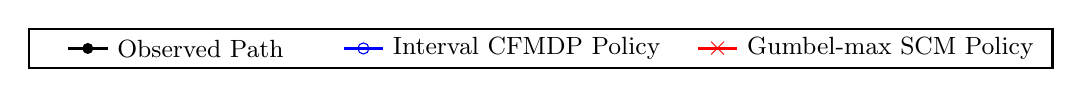
\begin{tikzpicture}[scale=1.0, every node/.style={scale=1.0}]
            \draw[thick, black] (-3, -0.25) rectangle (10, 0.25);
            %
            \draw[black, line width=1pt] (-2.5, 0.0) -- (-2,0.0);
            \fill[black] (-2.25,0.0) circle (2pt); %
            \node[right] at (-2,0.0) {\small Observed Path};
            
            %
            \draw[blue, line width=1pt] (1.0,0.0) -- (1.5,0.0);
            \node[draw=blue, circle, minimum size=4pt, inner sep=0pt] at (1.25,0.0) {}; %
            \node[right] at (1.5,0.0) {\small Interval CFMDP Policy};
            
            %
            \draw[red, line width=1pt] (5.5,0) -- (6,0);
            \node[red] at (5.75,0) {$\boldsymbol{\times}$}; %
            \node[right] at (6,0) {\small Gumbel-max SCM Policy};
        \end{tikzpicture}
    }\\
    %
    \subfigure[\footnotesize Lowest cumulative reward: Interval CFMDP ($312$), Gumbel-max SCM ($312$)]{%
        \resizebox{0.76\columnwidth}{!}{
             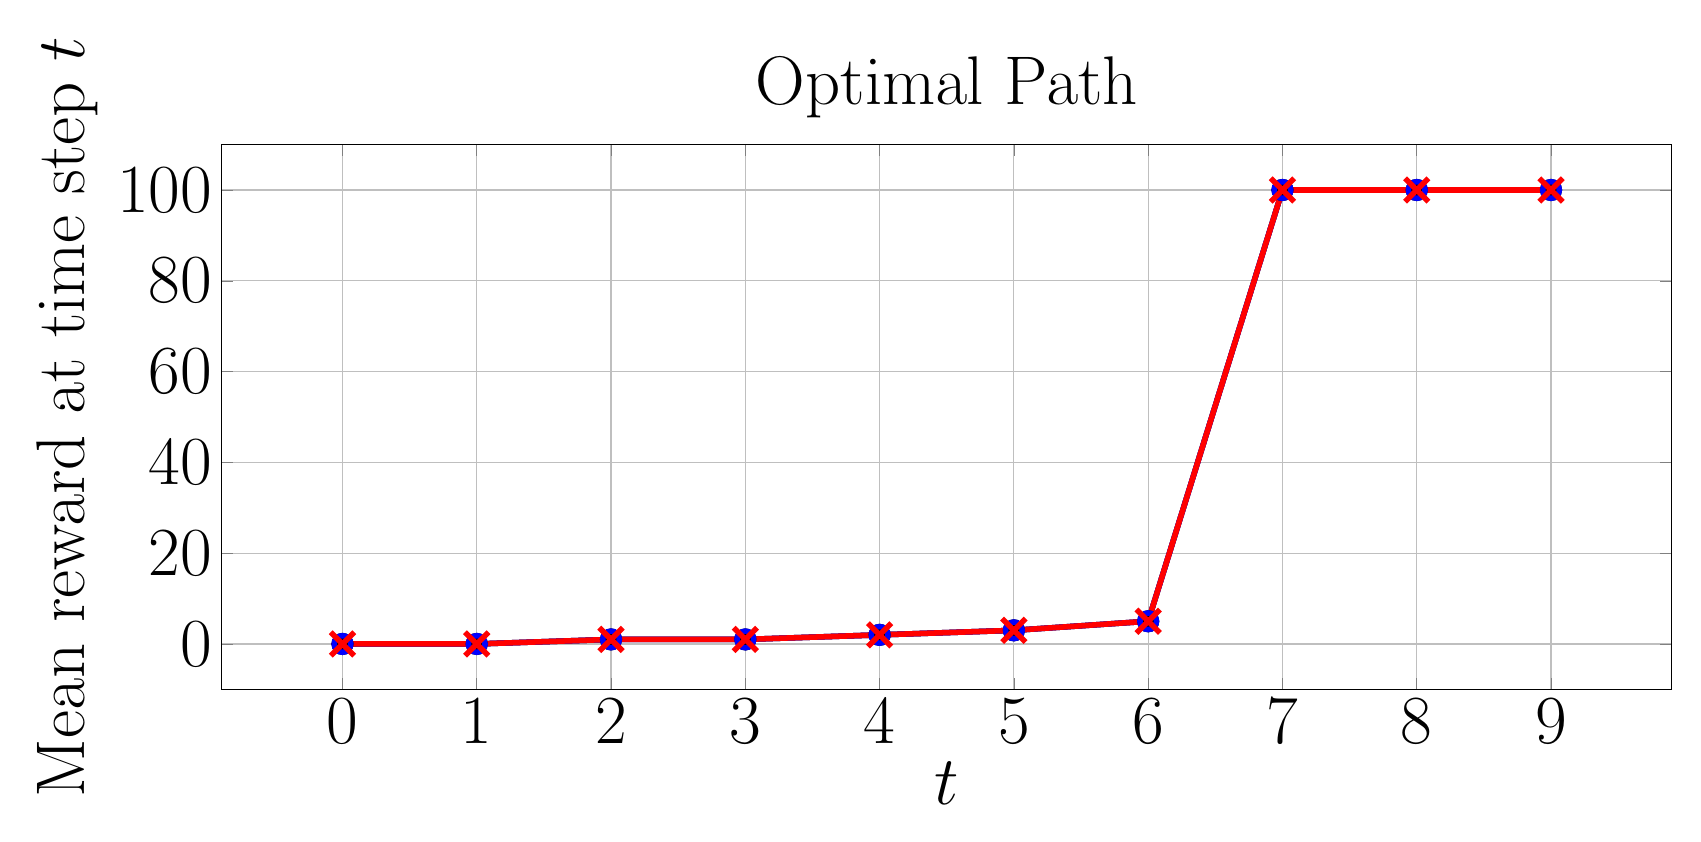
\begin{tikzpicture}
                \begin{axis}[
                    xlabel={$t$},
                    ylabel={Mean reward at time step $t$},
                    title={Optimal Path},
                    grid=both,
                    width=20cm, height=8.5cm,
                    every axis/.style={font=\Huge},
                    %
                ]
                \addplot[
                    color=black, %
                    mark=*, %
                    line width=2pt,
                    mark size=3pt,
                    error bars/.cd,
                    y dir=both, %
                    y explicit, %
                    error bar style={line width=1pt,solid},
                    error mark options={line width=1pt,mark size=4pt,rotate=90}
                ]
                coordinates {
                    (0, 0.0)  +- (0, 0.0)
                    (1, 0.0)  +- (0, 0.0) 
                    (2, 1.0)  +- (0, 0.0) 
                    (3, 1.0)  +- (0, 0.0)
                    (4, 2.0)  +- (0, 0.0)
                    (5, 3.0) +- (0, 0.0)
                    (6, 5.0) +- (0, 0.0)
                    (7, 100.0) +- (0, 0.0)
                    (8, 100.0) +- (0, 0.0)
                    (9, 100.0) +- (0, 0.0)
                };
                %
                \addplot[
                    color=blue, %
                    mark=o, %
                    line width=2pt,
                    mark size=3pt,
                    error bars/.cd,
                    y dir=both, %
                    y explicit, %
                    error bar style={line width=1pt,solid},
                    error mark options={line width=1pt,mark size=4pt,rotate=90}
                ]
                 coordinates {
                    (0, 0.0)  +- (0, 0.0)
                    (1, 0.0)  +- (0, 0.0) 
                    (2, 1.0)  +- (0, 0.0) 
                    (3, 1.0)  +- (0, 0.0)
                    (4, 2.0)  +- (0, 0.0)
                    (5, 3.0) +- (0, 0.0)
                    (6, 5.0) +- (0, 0.0)
                    (7, 100.0) +- (0, 0.0)
                    (8, 100.0) +- (0, 0.0)
                    (9, 100.0) +- (0, 0.0)
                };
                %
                \addplot[
                    color=red, %
                    mark=x, %
                    line width=2pt,
                    mark size=6pt,
                    error bars/.cd,
                    y dir=both, %
                    y explicit, %
                    error bar style={line width=1pt,solid},
                    error mark options={line width=1pt,mark size=4pt,rotate=90}
                ]
                coordinates {
                    (0, 0.0)  +- (0, 0.0)
                    (1, 0.0)  +- (0, 0.0) 
                    (2, 1.0)  +- (0, 0.0) 
                    (3, 1.0)  +- (0, 0.0)
                    (4, 2.0)  +- (0, 0.0)
                    (5, 3.0) +- (0, 0.0)
                    (6, 5.0) +- (0, 0.0)
                    (7, 100.0) +- (0, 0.0)
                    (8, 100.0) +- (0, 0.0)
                    (9, 100.0) +- (0, 0.0)
                };
                \end{axis}
            \end{tikzpicture}
         }
    }
    \hspace{1cm}
    \subfigure[\footnotesize Lowest cumulative reward: Interval CFMDP ($19$), Gumbel-max SCM ($-88$)]{%
         \resizebox{0.76\columnwidth}{!}{
            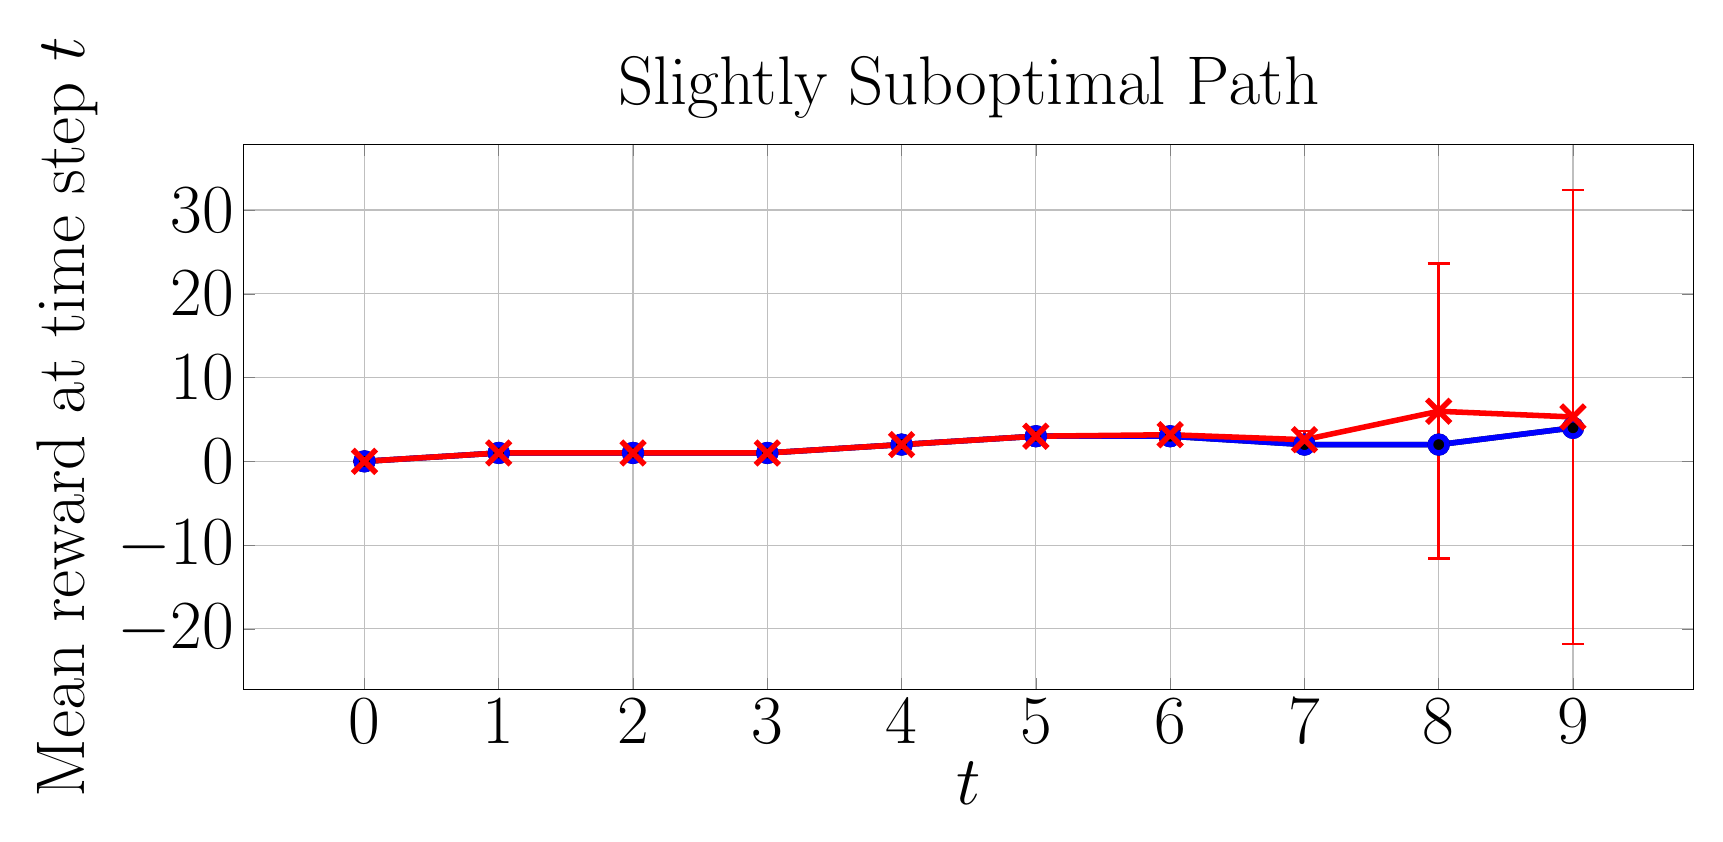
\begin{tikzpicture}
                \begin{axis}[
                    xlabel={$t$},
                    ylabel={Mean reward at time step $t$},
                    title={Slightly Suboptimal Path},
                    grid=both,
                    width=20cm, height=8.5cm,
                    every axis/.style={font=\Huge},
                    %
                ]
                \addplot[
                    color=black, %
                    mark=*, %
                    line width=2pt,
                    mark size=3pt,
                    error bars/.cd,
                    y dir=both, %
                    y explicit, %
                    error bar style={line width=1pt,solid},
                    error mark options={line width=1pt,mark size=4pt,rotate=90}
                ]
              coordinates {
                    (0, 0.0)  +- (0, 0.0)
                    (1, 1.0)  +- (0, 0.0) 
                    (2, 1.0)  +- (0, 0.0) 
                    (3, 1.0)  +- (0, 0.0)
                    (4, 2.0)  +- (0, 0.0)
                    (5, 3.0) +- (0, 0.0)
                    (6, 3.0) +- (0, 0.0)
                    (7, 2.0) +- (0, 0.0)
                    (8, 2.0) +- (0, 0.0)
                    (9, 4.0) +- (0, 0.0)
                };
                %
                \addplot[
                    color=blue, %
                    mark=o, %
                    line width=2pt,
                    mark size=3pt,
                    error bars/.cd,
                    y dir=both, %
                    y explicit, %
                    error bar style={line width=1pt,solid},
                    error mark options={line width=1pt,mark size=4pt,rotate=90}
                ]
              coordinates {
                    (0, 0.0)  +- (0, 0.0)
                    (1, 1.0)  +- (0, 0.0) 
                    (2, 1.0)  +- (0, 0.0) 
                    (3, 1.0)  +- (0, 0.0)
                    (4, 2.0)  +- (0, 0.0)
                    (5, 3.0) +- (0, 0.0)
                    (6, 3.0) +- (0, 0.0)
                    (7, 2.0) +- (0, 0.0)
                    (8, 2.0) +- (0, 0.0)
                    (9, 4.0) +- (0, 0.0)
                };
                %
                \addplot[
                    color=red, %
                    mark=x, %
                    line width=2pt,
                    mark size=6pt,
                    error bars/.cd,
                    y dir=both, %
                    y explicit, %
                    error bar style={line width=1pt,solid},
                    error mark options={line width=1pt,mark size=4pt,rotate=90}
                ]
                coordinates {
                    (0, 0.0)  +- (0, 0.0)
                    (1, 1.0)  +- (0, 0.0) 
                    (2, 1.0)  +- (0, 0.0) 
                    (3, 1.0)  +- (0, 0.0)
                    (4, 2.0)  += (0, 0.0)
                    (5, 3.0)  += (0, 0.0)
                    (6, 3.17847) += (0, 0.62606746) -= (0, 0.62606746)
                    (7, 2.5832885) += (0, 1.04598233) -= (0, 1.04598233)
                    (8, 5.978909) += (0, 17.60137623) -= (0, 17.60137623)
                    (9, 5.297059) += (0, 27.09227512) -= (0, 27.09227512)
                };
                \end{axis}
            \end{tikzpicture}
         }
    }\\[-1.5pt]
    \subfigure[\footnotesize Lowest cumulative reward: Interval CFMDP ($14$), Gumbel-max SCM ($-598$)]{%
         \resizebox{0.76\columnwidth}{!}{
             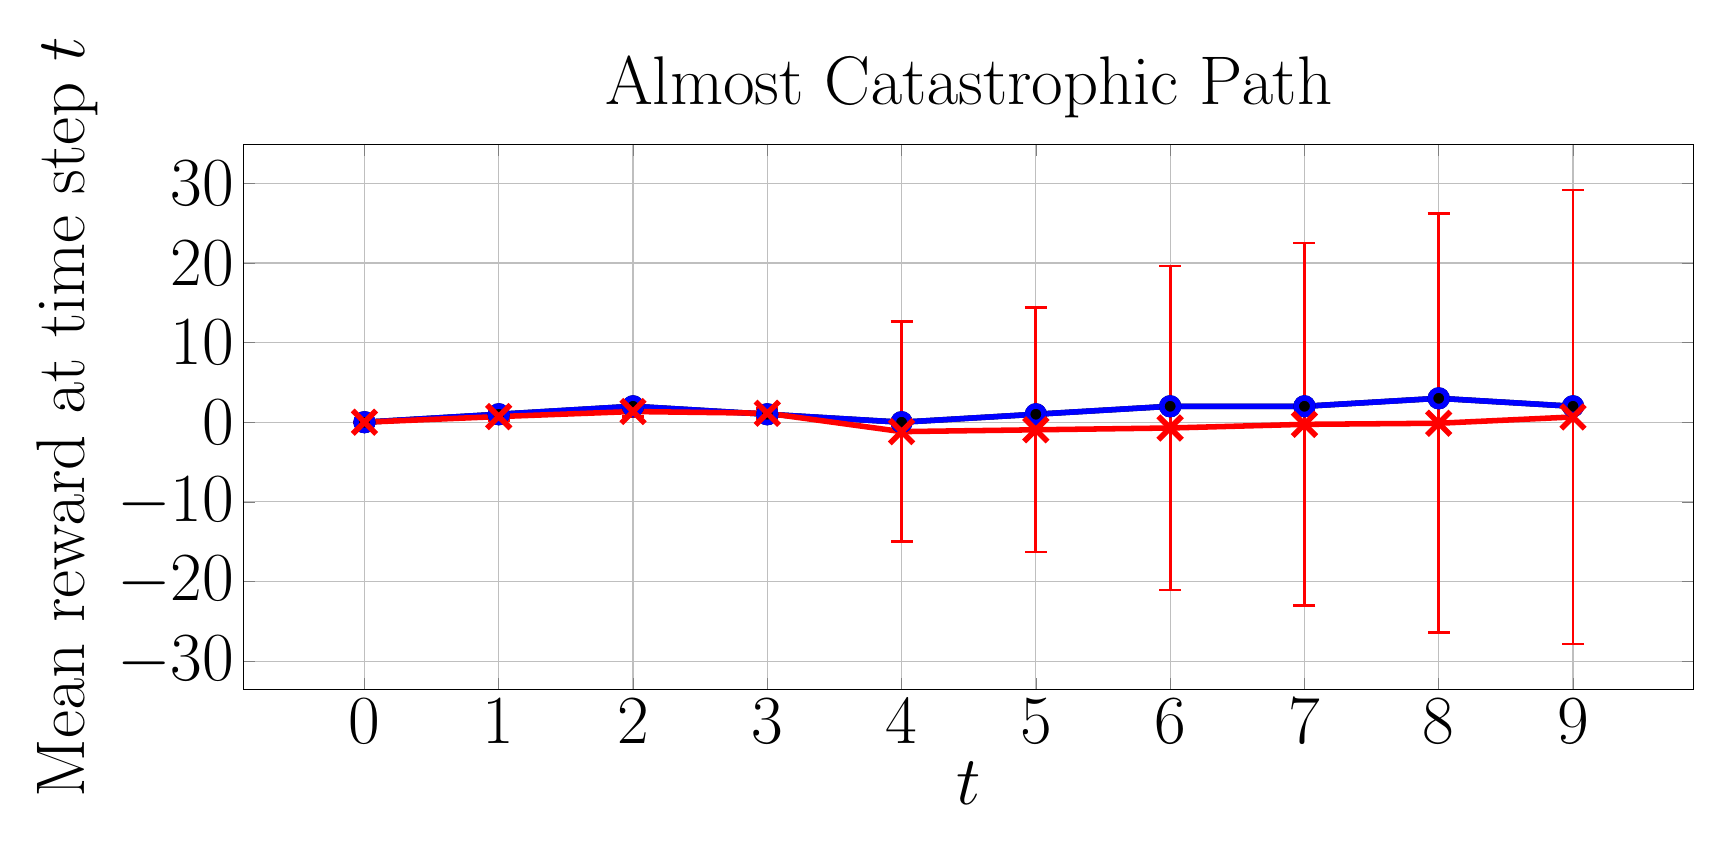
\begin{tikzpicture}
                \begin{axis}[
                    xlabel={$t$},
                    ylabel={Mean reward at time step $t$},
                    title={Almost Catastrophic Path},
                    grid=both,
                    width=20cm, height=8.5cm,
                    every axis/.style={font=\Huge},
                    %
                ]
                \addplot[
                    color=black, %
                    mark=*, %
                    line width=2pt,
                    mark size=3pt,
                    error bars/.cd,
                    y dir=both, %
                    y explicit, %
                    error bar style={line width=1pt,solid},
                    error mark options={line width=1pt,mark size=4pt,rotate=90}
                ]
                coordinates {
                    (0, 0.0)  +- (0, 0.0)
                    (1, 1.0)  +- (0, 0.0) 
                    (2, 2.0)  +- (0, 0.0) 
                    (3, 1.0)  +- (0, 0.0)
                    (4, 0.0)  +- (0, 0.0)
                    (5, 1.0) +- (0, 0.0)
                    (6, 2.0) +- (0, 0.0)
                    (7, 2.0) +- (0, 0.0)
                    (8, 3.0) +- (0, 0.0)
                    (9, 2.0) +- (0, 0.0)
                };
                %
                \addplot[
                    color=blue, %
                    mark=o, %
                    line width=2pt,
                    mark size=3pt,
                    error bars/.cd,
                    y dir=both, %
                    y explicit, %
                    error bar style={line width=1pt,solid},
                    error mark options={line width=1pt,mark size=4pt,rotate=90}
                ]
                coordinates {
                    (0, 0.0)  +- (0, 0.0)
                    (1, 1.0)  +- (0, 0.0) 
                    (2, 2.0)  +- (0, 0.0) 
                    (3, 1.0)  +- (0, 0.0)
                    (4, 0.0)  +- (0, 0.0)
                    (5, 1.0) +- (0, 0.0)
                    (6, 2.0) +- (0, 0.0)
                    (7, 2.0) +- (0, 0.0)
                    (8, 3.0) +- (0, 0.0)
                    (9, 2.0) +- (0, 0.0)
                };
                %
                \addplot[
                    color=red, %
                    mark=x, %
                    line width=2pt,
                    mark size=6pt,
                    error bars/.cd,
                    y dir=both, %
                    y explicit, %
                    error bar style={line width=1pt,solid},
                    error mark options={line width=1pt,mark size=4pt,rotate=90}
                ]
                coordinates {
                    (0, 0.0)  +- (0, 0.0)
                    (1, 0.7065655)  +- (0, 0.4553358) 
                    (2, 1.341673)  +- (0, 0.67091621) 
                    (3, 1.122926)  +- (0, 0.61281824)
                    (4, -1.1821935)  +- (0, 13.82444042)
                    (5, -0.952399)  +- (0, 15.35195457)
                    (6, -0.72672) +- (0, 20.33508414)
                    (7, -0.268983) +- (0, 22.77861454)
                    (8, -0.1310835) +- (0, 26.31013314)
                    (9, 0.65806) +- (0, 28.50670214)
                };
                %
            %
            %
            %
            %
            %
            %
            %
            %
            %
            %
            %
            %
            %
            %
            %
            %
            %
            %
                \end{axis}
            \end{tikzpicture}
         }
    }
    \hspace{1cm}
    \subfigure[\footnotesize Lowest cumulative reward: Interval CFMDP ($-698$), Gumbel-max SCM ($-698$)]{%
         \resizebox{0.76\columnwidth}{!}{
            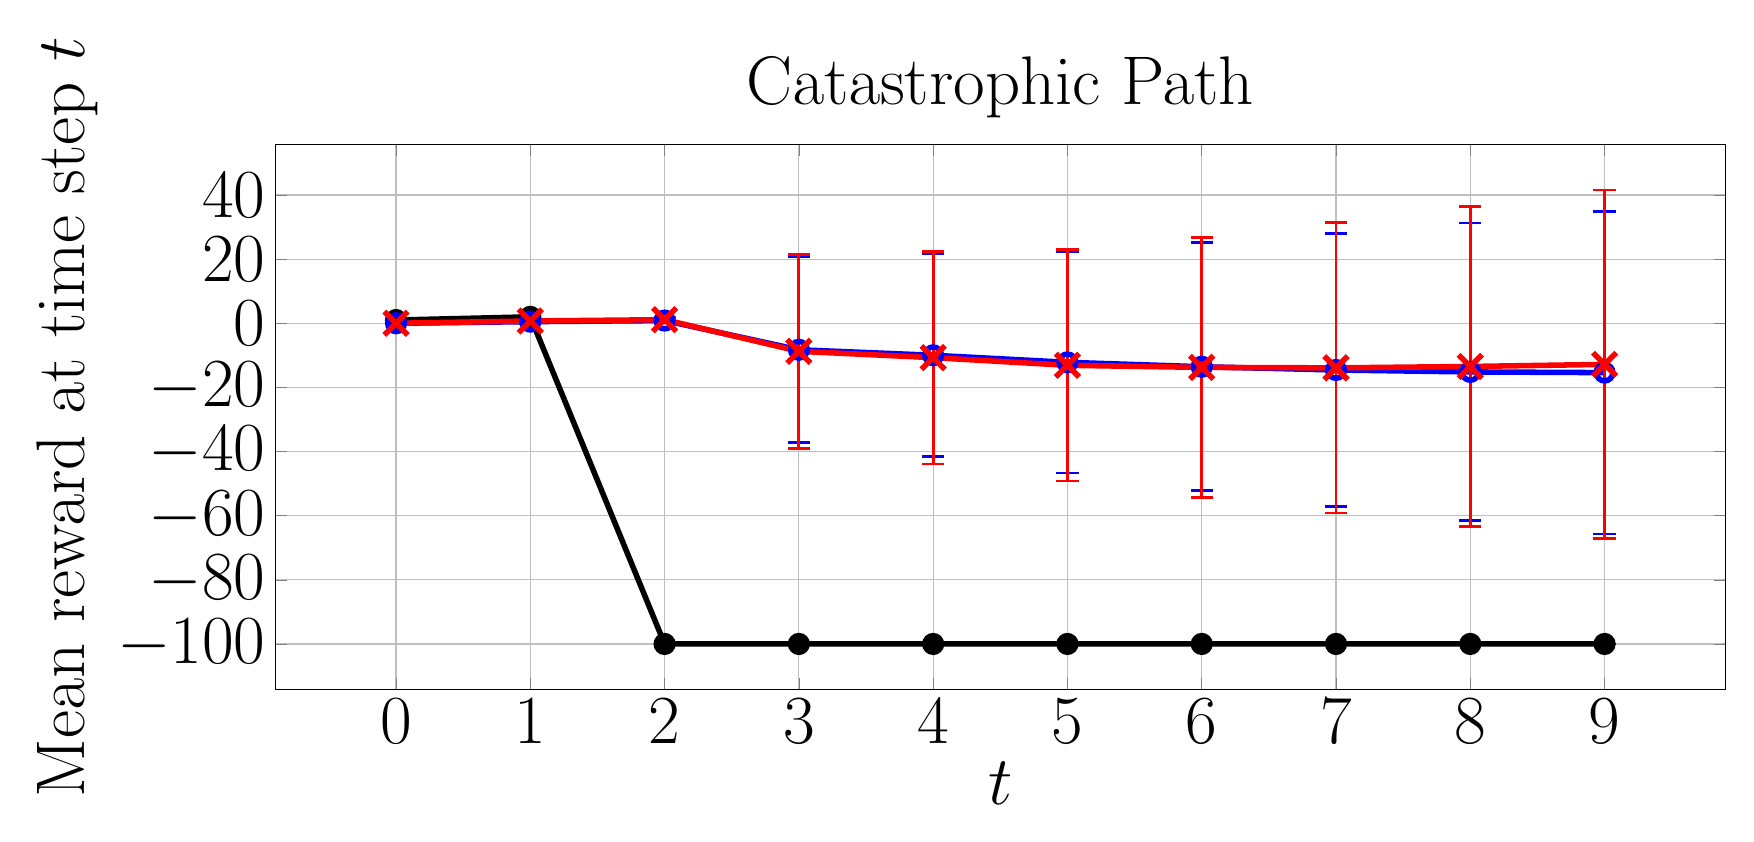
\begin{tikzpicture}
                \begin{axis}[
                    xlabel={$t$},
                    ylabel={Mean reward at time step $t$},
                    title={Catastrophic Path},
                    grid=both,
                    width=20cm, height=8.5cm,
                    every axis/.style={font=\Huge},
                    %
                ]
                \addplot[
                    color=black, %
                    mark=*, %
                    line width=2pt,
                    mark size=3pt,
                    error bars/.cd,
                    y dir=both, %
                    y explicit, %
                    error bar style={line width=1pt,solid},
                    error mark options={line width=1pt,mark size=4pt,rotate=90}
                ]
                coordinates {
                    (0, 1.0)  +- (0, 0.0)
                    (1, 2.0)  +- (0, 0.0) 
                    (2, -100.0)  +- (0, 0.0) 
                    (3, -100.0)  +- (0, 0.0)
                    (4, -100.0)  +- (0, 0.0)
                    (5, -100.0) +- (0, 0.0)
                    (6, -100.0) +- (0, 0.0)
                    (7, -100.0) +- (0, 0.0)
                    (8, -100.0) +- (0, 0.0)
                    (9, -100.0) +- (0, 0.0)
                };
                %
                \addplot[
                    color=blue, %
                    mark=o, %
                    line width=2pt,
                    mark size=3pt,
                    error bars/.cd,
                    y dir=both, %
                    y explicit, %
                    error bar style={line width=1pt,solid},
                    error mark options={line width=1pt,mark size=4pt,rotate=90}
                ]
                coordinates {
                    (0, 0.0)  +- (0, 0.0)
                    (1, 0.504814)  +- (0, 0.49997682) 
                    (2, 0.8439835)  +- (0, 0.76831917) 
                    (3, -8.2709165)  +- (0, 28.93656754)
                    (4, -9.981082)  +- (0, 31.66825363)
                    (5, -12.1776325) +- (0, 34.53463233)
                    (6, -13.556076) +- (0, 38.62845372)
                    (7, -14.574418) +- (0, 42.49603359)
                    (8, -15.1757075) +- (0, 46.41913968)
                    (9, -15.3900395) +- (0, 50.33563368)
                };
                %
                \addplot[
                    color=red, %
                    mark=x, %
                    line width=2pt,
                    mark size=6pt,
                    error bars/.cd,
                    y dir=both, %
                    y explicit, %
                    error bar style={line width=1pt,solid},
                    error mark options={line width=1pt,mark size=4pt,rotate=90}
                ]
                coordinates {
                    (0, 0.0)  +- (0, 0.0)
                    (1, 0.701873)  +- (0, 0.45743556) 
                    (2, 1.1227805)  +- (0, 0.73433129) 
                    (3, -8.7503255)  +- (0, 30.30257976)
                    (4, -10.722092)  +- (0, 33.17618589)
                    (5, -13.10721)  +- (0, 36.0648089)
                    (6, -13.7631645) +- (0, 40.56553451)
                    (7, -13.909043) +- (0, 45.23829402)
                    (8, -13.472517) +- (0, 49.96270296)
                    (9, -12.8278835) +- (0, 54.38618735)
                };
                %
            %
            %
            %
            %
            %
            %
            %
            %
            %
            %
            %
            %
            %
            %
            %
            %
            %
            %
                \end{axis}
            \end{tikzpicture}
         }
    }
    \caption{Average instant reward of CF paths induced by policies on GridWorld $p=0.4$.}
    \label{fig: reward p=0.4}
\end{figure*}

\subsection{Experimental Setup}
To compare policy performance, we measure the average rewards of counterfactual paths induced by our policy and the Gumbel-max policy by uniformly sampling $200$ counterfactual MDPs from the ICFMDP and generating $10,000$ counterfactual paths over each sampled CFMDP. \jl{Since the interval CFMDP depends on the observed path, we select $4$  paths of varying optimality to evaluate how the observed path impacts the performance of both policies: an optimal path, a slightly suboptimal path that could reach the optimal reward with a few changes, a catastrophic path that enters a catastrophic, terminal state with low reward, and an almost catastrophic path that was close to entering a catastrophic state.} When measuring the average probability bound widths and execution time needed to generate the ICFMDPs, we averaged over $20$ randomly generated observed paths
\footnote{Further training details are provided in Appendix \ref{app: training details}, and the code is provided at \href{https://github.com/ddv-lab/robust-cf-inference-in-MDPs}{https://github.com/ddv-lab/robust-cf-inference-in-MDPs}
%
%
.}.

\subsection{GridWorld}
\jl{The GridWorld MDP is a $4 \times 4$ grid where an agent must navigate from the top-left corner to the goal state in the bottom-right corner, avoiding a dangerous terminal state in the centre. At each time step, the agent can move up, down, left, or right, but there is a small probability (controlled by hyper-parameter $p$) of moving in an unintended direction. As the agent nears the goal, the reward for each state increases, culminating in a reward of $+100$ for reaching the goal. Entering the dangerous state results in a penalty of $-100$. We use two versions of GridWorld: a less stochastic version with $p=0.9$ (i.e., $90$\% chance of moving in the chosen direction) and a more stochastic version with $p=0.4$.}

\paragraph{GridWorld ($p=0.9$)}
When $p=0.9$, the counterfactual probability bounds are typically narrow (see Table \ref{tab:nonzero_probs} for average measurements). Consequently, as shown in Figure \ref{fig: reward p=0.9}, both policies are nearly identical and perform similarly well across the optimal, slightly suboptimal, and catastrophic paths.
%
However, for the almost catastrophic path, the interval CFMDP path is more conservative and follows the observed path more closely (as this is where the probability bounds are narrowest), which typically requires one additional step to reach the goal state than the Gumbel-max SCM policy.
%

\paragraph{GridWorld ($p=0.4$)}
\jl{When $p=0.4$, the GridWorld environment becomes more uncertain, increasing the risk of entering the dangerous state even if correct actions are chosen. Thus, as shown in Figure \ref{fig: reward p=0.4}, the interval CFMDP policy adopts a more conservative approach, avoiding deviation from the observed policy if it cannot guarantee higher counterfactual rewards (see the slightly suboptimal and almost catastrophic paths), whereas the Gumbel-max SCM is inconsistent: it can yield higher rewards, but also much lower rewards, reflected in the wide error bars.} For the catastrophic path, both policies must deviate from the observed path to achieve a higher reward and, in this case, perform similarly.
%
%
%
%
\subsection{Sepsis}
The Sepsis MDP \citep{oberst2019counterfactual} simulates trajectories of Sepsis patients. Each state consists of four vital signs (heart rate, blood pressure, oxygen concentration, and glucose levels), categorised as low, normal, or high.
and three treatments that can be toggled on/off at each time step (8 actions in total). Unlike \citet{oberst2019counterfactual}, we scale rewards based on the number of out-of-range vital signs, between $-1000$ (patient dies) and $1000$ (patient discharged). \jl{Like the GridWorld $p=0.4$ experiment, the Sepsis MDP is highly uncertain, as many states are equally likely to lead to optimal and poor outcomes. Thus, as shown in Figure \ref{fig: reward sepsis}, both policies follow the observed optimal and almost catastrophic paths to guarantee rewards are no worse than the observation.} However, improving the catastrophic path requires deviating from the observation. Here, the Gumbel-max SCM policy, on average, performs better than the interval CFMDP policy. But, since both policies have lower bounds clipped at $-1000$, neither policy reliably improves over the observation. In contrast, for the slightly suboptimal path, the interval CFMDP policy performs significantly better, shown by its higher lower bounds. 
Moreover, in these two cases, the worst-case counterfactual path generated by the interval CFMDP policy is better than that of the Gumbel-max SCM policy,
indicating its greater robustness.
%
\begin{figure*}
    \centering
     \resizebox{0.6\textwidth}{!}{
        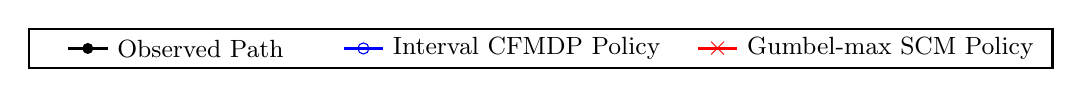
\begin{tikzpicture}[scale=1.0, every node/.style={scale=1.0}]
            \draw[thick, black] (-3, -0.25) rectangle (10, 0.25);
            %
            \draw[black, line width=1pt] (-2.5, 0.0) -- (-2,0.0);
            \fill[black] (-2.25,0.0) circle (2pt); %
            \node[right] at (-2,0.0) {\small Observed Path};
            
            %
            \draw[blue, line width=1pt] (1.0,0.0) -- (1.5,0.0);
            \node[draw=blue, circle, minimum size=4pt, inner sep=0pt] at (1.25,0.0) {}; %
            \node[right] at (1.5,0.0) {\small Interval CFMDP Policy};
            
            %
            \draw[red, line width=1pt] (5.5,0) -- (6,0);
            \node[red] at (5.75,0) {$\boldsymbol{\times}$}; %
            \node[right] at (6,0) {\small Gumbel-max SCM Policy};
        \end{tikzpicture}
    }\\
    \subfigure[\footnotesize Lowest cumulative reward: Interval CFMDP ($8000$), Gumbel-max SCM ($8000$)]{%
         \resizebox{0.76\columnwidth}{!}{
             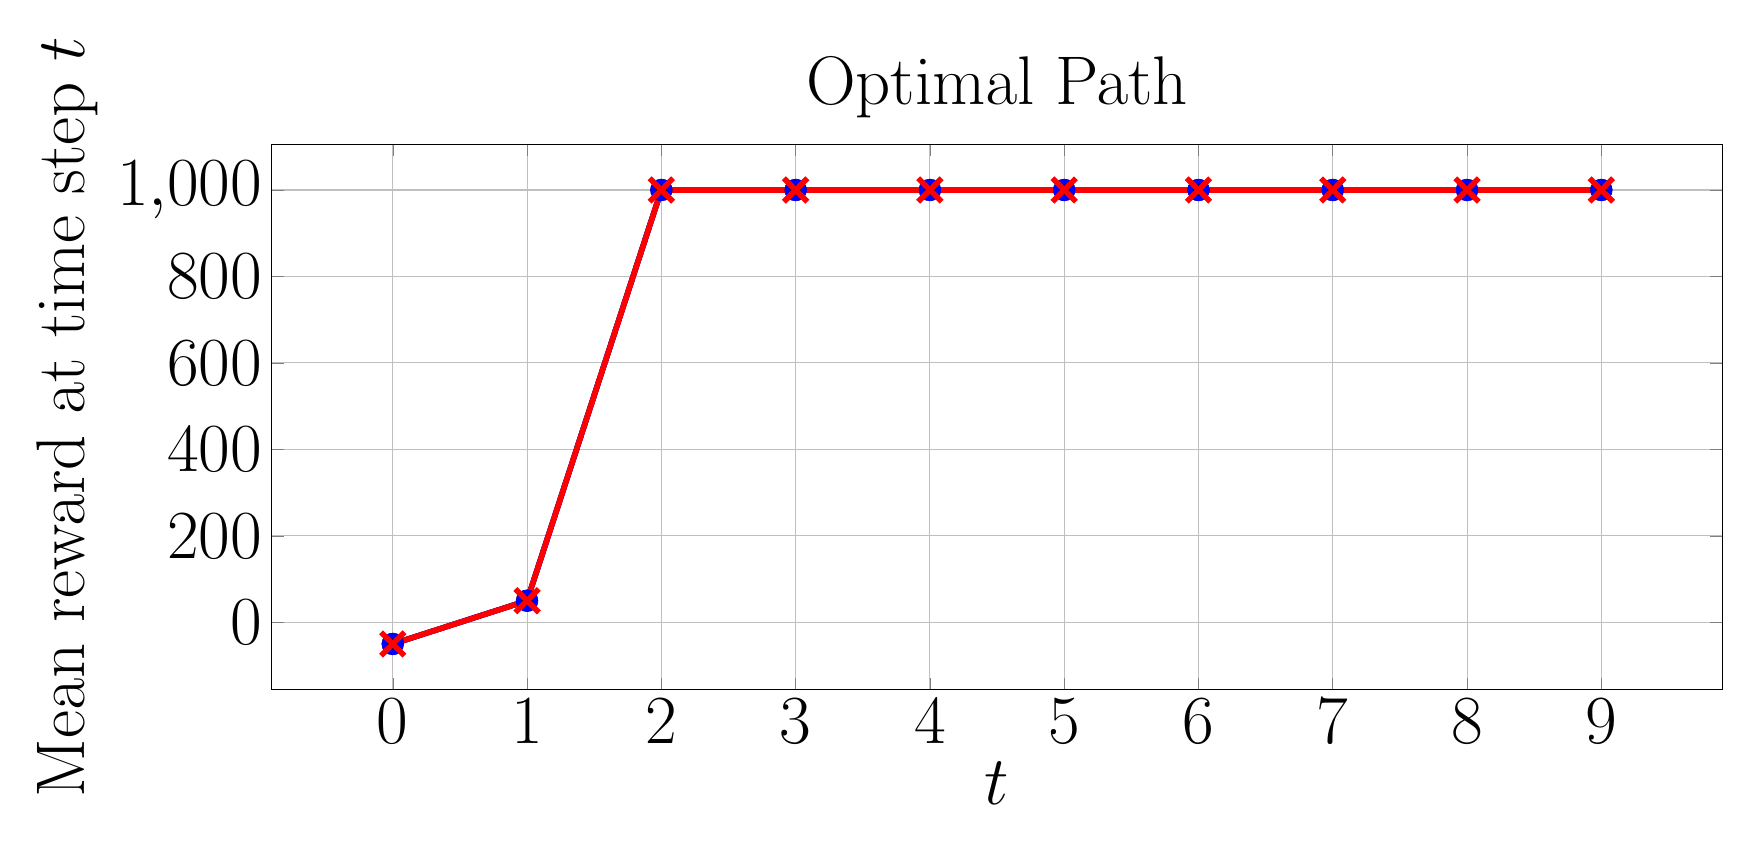
\begin{tikzpicture}
                \begin{axis}[
                    xlabel={$t$},
                    ylabel={Mean reward at time step $t$},
                    title={Optimal Path},
                    grid=both,
                    width=20cm, height=8.5cm,
                    every axis/.style={font=\Huge},
                    %
                ]
                \addplot[
                    color=black, %
                    mark=*, %
                    line width=2pt,
                    mark size=3pt,
                ]
                coordinates {
                    (0, -50.0)
                    (1, 50.0)
                    (2, 1000.0)
                    (3, 1000.0)
                    (4, 1000.0)
                    (5, 1000.0)
                    (6, 1000.0)
                    (7, 1000.0)
                    (8, 1000.0)
                    (9, 1000.0)
                };
                %
                \addplot[
                    color=blue, %
                    mark=o, %
                    line width=2pt,
                    mark size=3pt,
                    error bars/.cd,
                    y dir=both, %
                    y explicit, %
                    error bar style={line width=1pt,solid},
                    error mark options={line width=1pt,mark size=4pt,rotate=90}
                ]
                coordinates {
                    (0, -50.0)  +- (0, 0.0)
                    (1, 50.0)  +- (0, 0.0) 
                    (2, 1000.0)  +- (0, 0.0) 
                    (3, 1000.0)  +- (0, 0.0)
                    (4, 1000.0)  +- (0, 0.0)
                    (5, 1000.0) +- (0, 0.0)
                    (6, 1000.0) +- (0, 0.0)
                    (7, 1000.0) +- (0, 0.0)
                    (8, 1000.0) +- (0, 0.0)
                    (9, 1000.0) +- (0, 0.0)
                };
                %
                \addplot[
                    color=red, %
                    mark=x, %
                    line width=2pt,
                    mark size=6pt,
                    error bars/.cd,
                    y dir=both, %
                    y explicit, %
                    error bar style={line width=1pt,solid},
                    error mark options={line width=1pt,mark size=4pt,rotate=90}
                ]
                coordinates {
                    (0, -50.0)  +- (0, 0.0)
                    (1, 50.0)  +- (0, 0.0) 
                    (2, 1000.0)  +- (0, 0.0) 
                    (3, 1000.0)  +- (0, 0.0)
                    (4, 1000.0)  +- (0, 0.0)
                    (5, 1000.0) +- (0, 0.0)
                    (6, 1000.0) +- (0, 0.0)
                    (7, 1000.0) +- (0, 0.0)
                    (8, 1000.0) +- (0, 0.0)
                    (9, 1000.0) +- (0, 0.0)
                };
                %
                \end{axis}
            \end{tikzpicture}
         }
    }
    \hspace{1cm}
    \subfigure[\footnotesize Lowest cumulative reward: Interval CFMDP ($-5980$), Gumbel-max SCM ($-8000$)]{%
         \resizebox{0.76\columnwidth}{!}{
            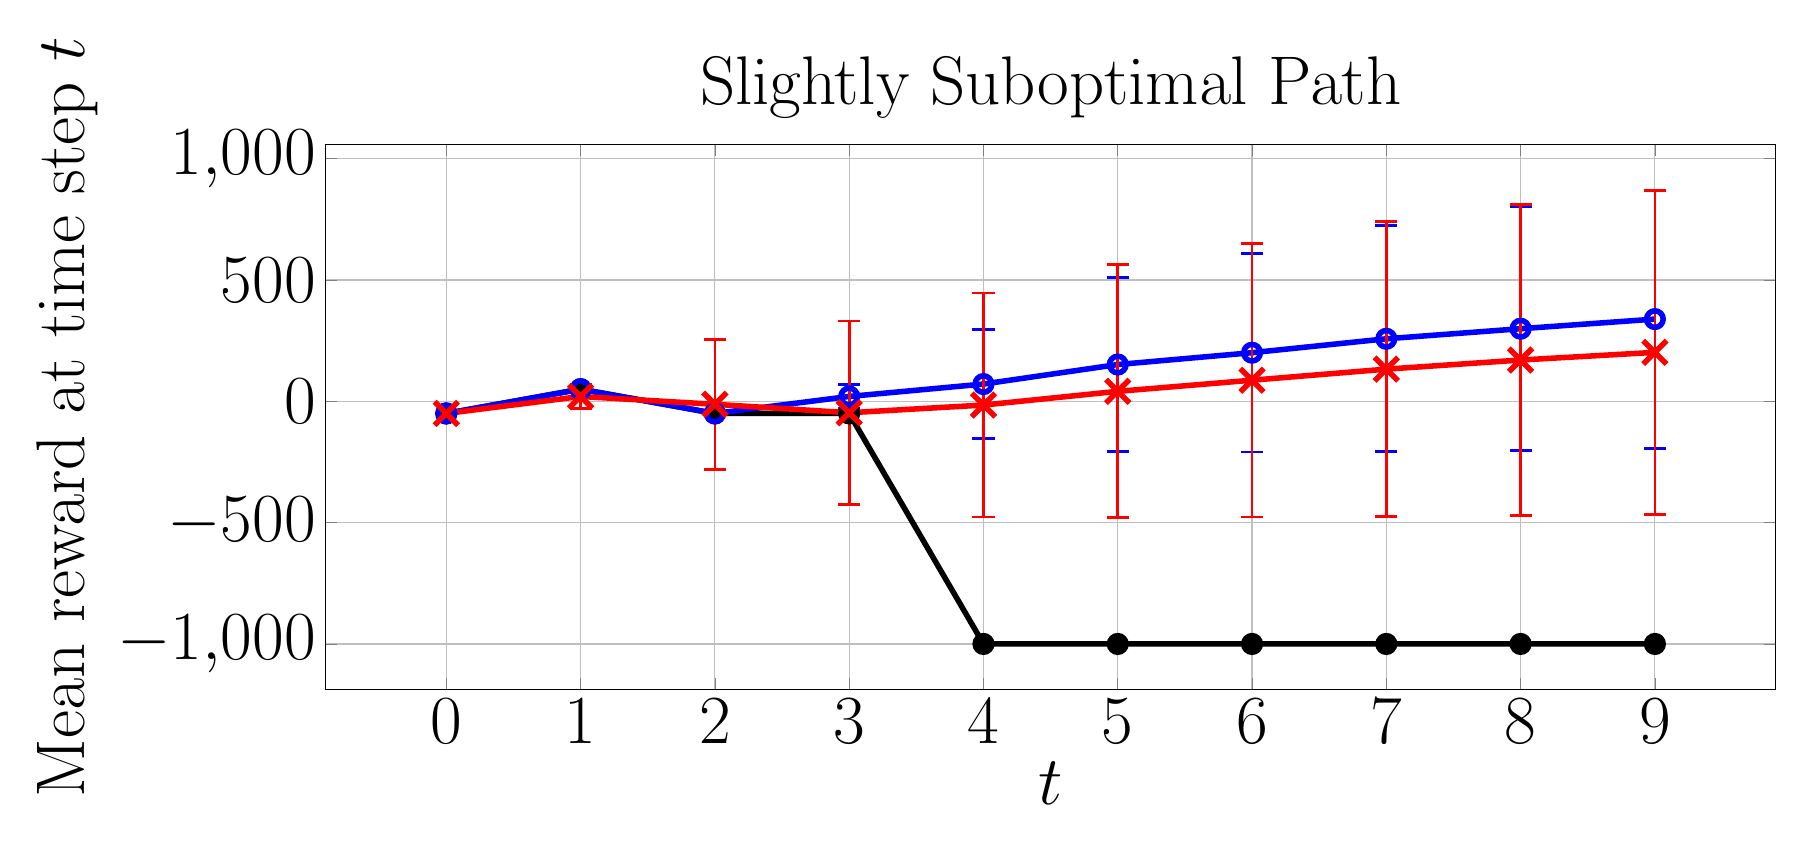
\begin{tikzpicture}
                \begin{axis}[
                    xlabel={$t$},
                    ylabel={Mean reward at time step $t$},
                    title={Slightly Suboptimal Path},
                    grid=both,
                    width=20cm, height=8.5cm,
                    every axis/.style={font=\Huge},
                    %
                ]
               \addplot[
                    color=black, %
                    mark=*, %
                    line width=2pt,
                    mark size=3pt,
                ]
                coordinates {
                    (0, -50.0)
                    (1, 50.0)
                    (2, -50.0)
                    (3, -50.0)
                    (4, -1000.0)
                    (5, -1000.0)
                    (6, -1000.0)
                    (7, -1000.0)
                    (8, -1000.0)
                    (9, -1000.0)
                };
                %
                \addplot[
                    color=blue, %
                    mark=o, %
                    line width=2pt,
                    mark size=3pt,
                    error bars/.cd,
                    y dir=both, %
                    y explicit, %
                    error bar style={line width=1pt,solid},
                    error mark options={line width=1pt,mark size=4pt,rotate=90}
                ]
                coordinates {
                    (0, -50.0)  +- (0, 0.0)
                    (1, 50.0)  +- (0, 0.0) 
                    (2, -50.0)  +- (0, 0.0) 
                    (3, 20.0631)  +- (0, 49.97539413)
                    (4, 71.206585)  +- (0, 226.02033693)
                    (5, 151.60797) +- (0, 359.23292559)
                    (6, 200.40593) +- (0, 408.86185176)
                    (7, 257.77948) +- (0, 466.10372804)
                    (8, 299.237465) +- (0, 501.82579506)
                    (9, 338.9129) +- (0, 532.06124996)
                };
                %
                \addplot[
                    color=red, %
                    mark=x, %
                    line width=2pt,
                    mark size=6pt,
                    error bars/.cd,
                    y dir=both, %
                    y explicit, %
                    error bar style={line width=1pt,solid},
                    error mark options={line width=1pt,mark size=4pt,rotate=90}
                ]
                coordinates {
                    (0, -50.0)  +- (0, 0.0)
                    (1, 20.00736)  +- (0, 49.99786741) 
                    (2, -12.282865)  +- (0, 267.598755) 
                    (3, -47.125995)  +- (0, 378.41755832)
                    (4, -15.381965)  +- (0, 461.77616558)
                    (5, 41.15459) +- (0, 521.53189262)
                    (6, 87.01595) +- (0, 564.22243126 )
                    (7, 132.62376) +- (0, 607.31338037)
                    (8, 170.168145) +- (0, 641.48013693)
                    (9, 201.813135) +- (0, 667.29441777)
                };
                %
                %
                %
                %
                %
                %
                %
                %
                %
                %
                %
                %
                %
                %
                %
                %
                %
                %
                %
                \end{axis}
            \end{tikzpicture}
         }
    }\\[-1.5pt]
    \subfigure[\footnotesize Lowest cumulative reward: Interval CFMDP ($100$), Gumbel-max SCM ($100$)]{%
         \resizebox{0.76\columnwidth}{!}{
             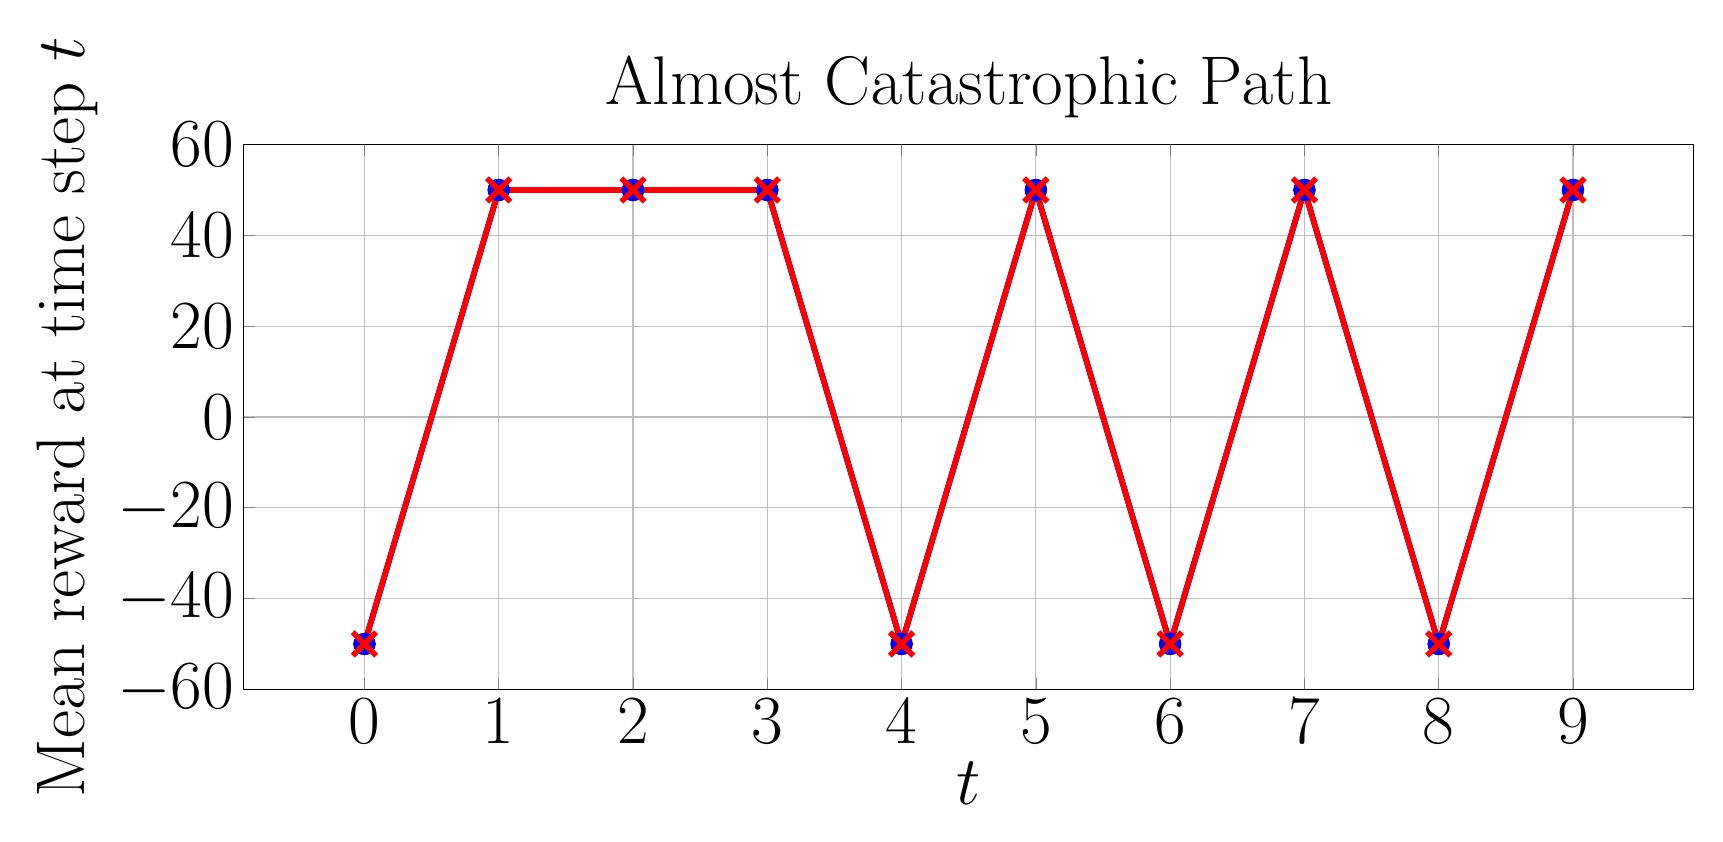
\begin{tikzpicture}
                \begin{axis}[
                    xlabel={$t$},
                    ylabel={Mean reward at time step $t$},
                    title={Almost Catastrophic Path},
                    grid=both,
                    every axis/.style={font=\Huge},
                    width=20cm, height=8.5cm,
                    %
                ]
               \addplot[
                    color=black, %
                    mark=*, %
                    line width=2pt,
                    mark size=3pt,
                ]
                coordinates {
                    (0, -50.0)
                    (1, 50.0)
                    (2, 50.0)
                    (3, 50.0)
                    (4, -50.0)
                    (5, 50.0)
                    (6, -50.0)
                    (7, 50.0)
                    (8, -50.0)
                    (9, 50.0)
                };
                %
                %
                \addplot[
                    color=blue, %
                    mark=o, %
                    line width=2pt,
                    mark size=3pt,
                    error bars/.cd,
                    y dir=both, %
                    y explicit, %
                    error bar style={line width=1pt,solid},
                    error mark options={line width=1pt,mark size=4pt,rotate=90}
                ]
                coordinates {
                    (0, -50.0)  +- (0, 0.0)
                    (1, 50.0)  +- (0, 0.0) 
                    (2, 50.0)  +- (0, 0.0) 
                    (3, 50.0)  +- (0, 0.0)
                    (4, -50.0)  +- (0, 0.0)
                    (5, 50.0) +- (0, 0.0)
                    (6, -50.0) +- (0, 0.0)
                    (7, 50.0) +- (0, 0.0)
                    (8, -50.0) +- (0, 0.0)
                    (9, 50.0) +- (0, 0.0)
                };
                %
                \addplot[
                    color=red, %
                    mark=x, %
                    line width=2pt,
                    mark size=6pt,
                    error bars/.cd,
                    y dir=both, %
                    y explicit, %
                    error bar style={line width=1pt,solid},
                    error mark options={line width=1pt,mark size=4pt,rotate=90}
                ]
                coordinates {
                    (0, -50.0)  +- (0, 0.0)
                    (1, 50.0)  +- (0, 0.0) 
                    (2, 50.0)  +- (0, 0.0) 
                    (3, 50.0)  +- (0, 0.0)
                    (4, -50.0)  +- (0, 0.0)
                    (5, 50.0) +- (0, 0.0)
                    (6, -50.0) +- (0, 0.0)
                    (7, 50.0) +- (0, 0.0)
                    (8, -50.0) +- (0, 0.0)
                    (9, 50.0) +- (0, 0.0)
                };
                %
                %
                %
                %
                %
                %
                %
                %
                %
                %
                %
                %
                %
                %
                %
                %
                %
                %
                %
                \end{axis}
            \end{tikzpicture}
         }
    }
    \hspace{1cm}
    \subfigure[\footnotesize Lowest cumulative reward: Interval CFMDP ($-7150$), Gumbel-max SCM ($-9050$)]{%
         \resizebox{0.76\columnwidth}{!}{
            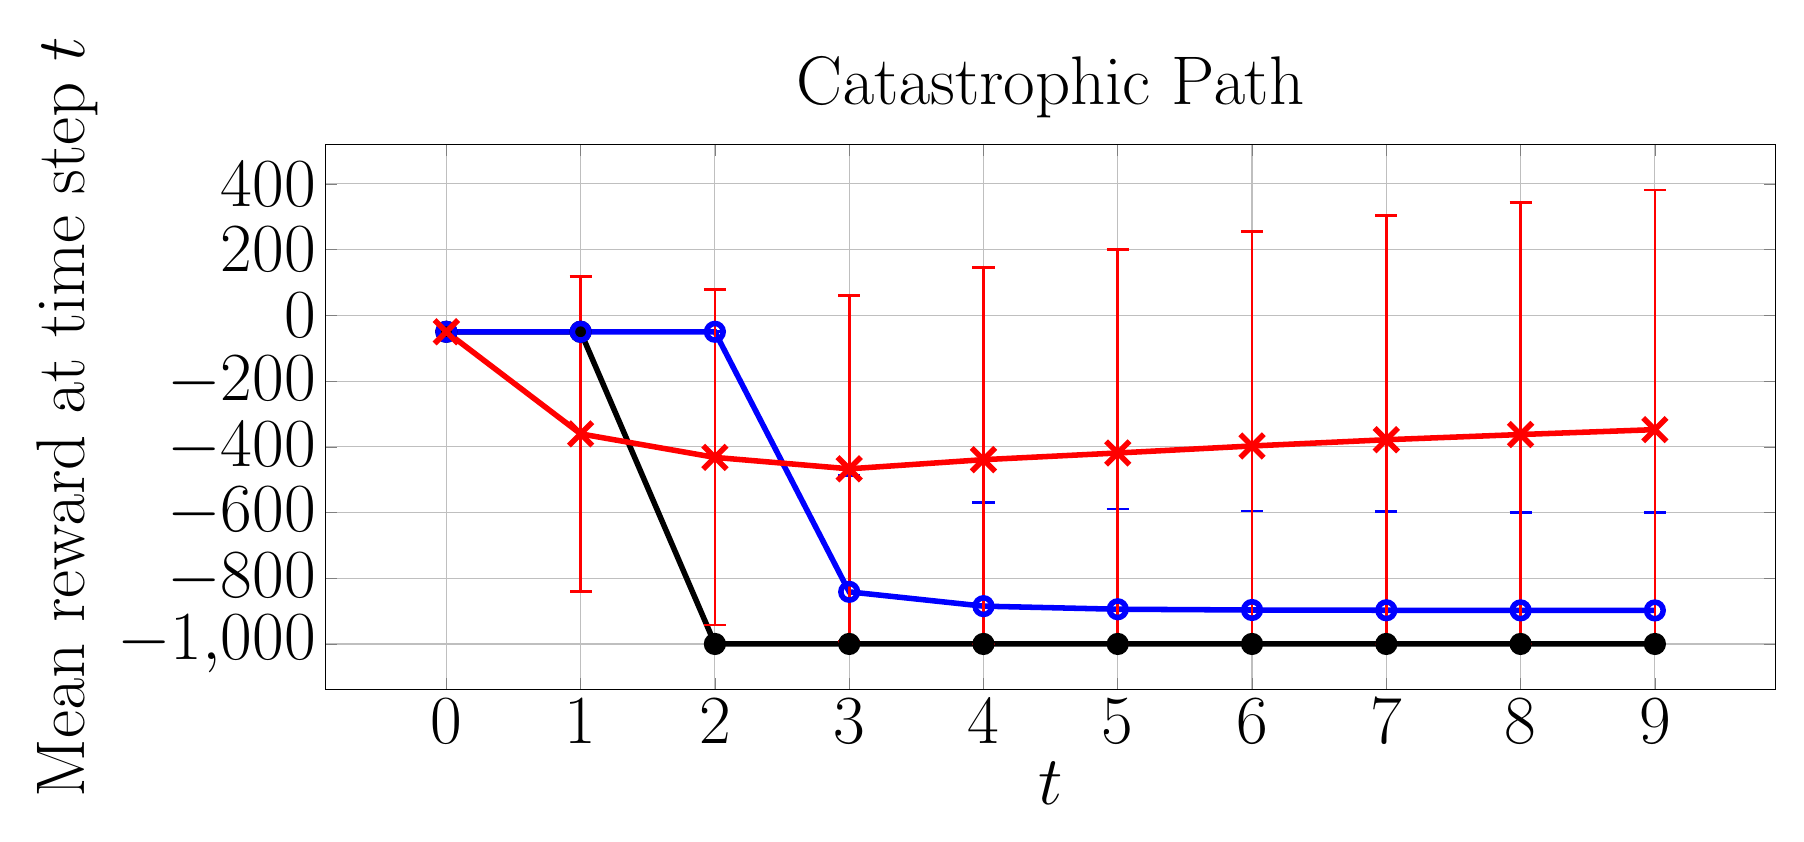
\begin{tikzpicture}
                \begin{axis}[
                    xlabel={$t$},
                    ylabel={Mean reward at time step $t$},
                    title={Catastrophic Path},
                    grid=both,
                    width=20cm, height=8.5cm,
                    every axis/.style={font=\Huge},
                    %
                ]
               \addplot[
                    color=black, %
                    mark=*, %
                    line width=2pt,
                    mark size=3pt,
                ]
                coordinates {
                    (0, -50.0)
                    (1, -50.0)
                    (2, -1000.0)
                    (3, -1000.0)
                    (4, -1000.0)
                    (5, -1000.0)
                    (6, -1000.0)
                    (7, -1000.0)
                    (8, -1000.0)
                    (9, -1000.0)
                };
                %
                %
                \addplot[
                    color=blue, %
                    mark=o, %
                    line width=2pt,
                    mark size=3pt,
                    error bars/.cd,
                    y dir=both, %
                    y explicit, %
                    error bar style={line width=1pt,solid},
                    error mark options={line width=1pt,mark size=4pt,rotate=90}
                ]
                coordinates {
                    (0, -50.0)  +- (0, 0.0)
                    (1, -50.0)  +- (0, 0.0) 
                    (2, -50.0)  +- (0, 0.0) 
                    (3, -841.440725)  += (0, 354.24605512) -= (0, 158.559275)
                    (4, -884.98225)  += (0, 315.37519669) -= (0, 115.01775)
                    (5, -894.330425) += (0, 304.88572805) -= (0, 105.669575)
                    (6, -896.696175) += (0, 301.19954514) -= (0, 103.303825)
                    (7, -897.4635) += (0, 299.61791279) -= (0, 102.5365)
                    (8, -897.77595) += (0, 298.80392585) -= (0, 102.22405)
                    (9, -897.942975) += (0, 298.32920557) -= (0, 102.057025)
                };
                %
                \addplot[
                    color=red, %
                    mark=x, %
                    line width=2pt,
                    mark size=6pt,
                    error bars/.cd,
                    y dir=both, %
                    y explicit, %
                    error bar style={line width=1pt,solid},
                    error mark options={line width=1pt,mark size=4pt,rotate=90}
                ]
            coordinates {
                    (0, -50.0)  +- (0, 0.0)
                    (1, -360.675265)  +- (0, 479.39812699) 
                    (2, -432.27629)  +- (0, 510.38620897) 
                    (3, -467.029545)  += (0, 526.36009628) -= (0, 526.36009628)
                    (4, -439.17429)  += (0, 583.96638919) -= (0, 560.82571)
                    (5, -418.82704) += (0, 618.43027478) -= (0, 581.17296)
                    (6, -397.464895) += (0, 652.67322574) -= (0, 602.535105)
                    (7, -378.49052) += (0, 682.85407033) -= (0, 621.50948)
                    (8, -362.654195) += (0, 707.01412023) -= (0, 637.345805)
                    (9, -347.737935) += (0, 729.29076479) -= (0, 652.262065)
                };
                %
                %
                %
                %
                %
                %
                %
                %
                %
                %
                %
                %
                %
                %
                %
                %
                %
                %
                %
                \end{axis}
            \end{tikzpicture}
         }
    }
    \caption{Average instant reward of CF paths induced by policies on Sepsis.}
    \label{fig: reward sepsis}
\end{figure*}

%
%
%
\subsection{Interval CFMDP Bounds}
%
%
Table \ref{tab:nonzero_probs} presents the mean counterfactual probability bound widths (excluding transitions where the upper bound is $0$) for each MDP, averaged over 20 observed paths. We compare the bounds under counterfactual stability (CS) and monotonicity (M) assumptions, CS alone, and no assumptions. This shows that the assumptions marginally reduce the bound widths, indicating the assumptions tighten the bounds without excluding too many causal models, as intended.
\renewcommand{\arraystretch}{1}

\begin{table}
\centering
\caption{Mean width of counterfactual probability bounds}
\resizebox{0.8\columnwidth}{!}{%
\begin{tabular}{|c|c|c|c|}
\hline
\multirow{2}{*}{\textbf{Environment}} & \multicolumn{3}{c|}{\textbf{Assumptions}} \\ \cline{2-4}
 & \textbf{CS + M} & \textbf{CS} & \textbf{None\tablefootnote{\jl{Equivalent to \citet{li2024probabilities}'s bounds (see Section \ref{sec: equivalence with Li}).}}} \\ \hline
\textbf{GridWorld} ($p=0.9$) & 0.0817 & 0.0977 & 0.100 \\ \hline
\textbf{GridWorld} ($p=0.4$) & 0.552  & 0.638  & 0.646 \\ \hline
\textbf{Sepsis} & 0.138 & 0.140 & 0.140 \\ \hline
\end{tabular}
}
\label{tab:nonzero_probs}
\end{table}


\subsection{Execution Times}
Table \ref{tab: times} compares the average time needed to generate the interval CFMDP vs.\ the Gumbel-max SCM CFMDP for 20 observations.
The GridWorld algorithms were run single-threaded, while the Sepsis experiments were run in parallel.
Generating the interval CFMDP is significantly faster as it uses exact analytical bounds, whereas the Gumbel-max CFMDP requires sampling from the Gumbel distribution to estimate counterfactual transition probabilities. \jl{Since constructing the counterfactual MDP models is the main bottleneck in both approaches, ours is more efficient overall and suitable for larger MDPs.}
\begin{table}
\centering
\caption{Mean execution time to generate CFMDPs}
\resizebox{0.99\columnwidth}{!}{%
\begin{tabular}{|c|c|c|}
\hline
\multirow{2}{*}{\textbf{Environment}} & \multicolumn{2}{c|}{\textbf{Mean Execution Time (s)}} \\ \cline{2-3} 
                                      & \textbf{Interval CFMDP} & \textbf{Gumbel-max CFMDP} \\ \hline
\textbf{GridWorld ($p=0.9$) }                  & 0.261                   & 56.1                      \\ \hline
\textbf{GridWorld ($p=0.4$)  }                 & 0.336                   & 54.5                      \\ \hline
\textbf{Sepsis}                                 & 688                     & 2940                      \\ \hline
\end{tabular}%
}
\label{tab: times}
\end{table}

\section{Conclusion}
In this work, we propose a simple yet effective approach, called SMILE, for graph few-shot learning with fewer tasks. Specifically, we introduce a novel dual-level mixup strategy, including within-task and across-task mixup, for enriching the diversity of nodes within each task and the diversity of tasks. Also, we incorporate the degree-based prior information to learn expressive node embeddings. Theoretically, we prove that SMILE effectively enhances the model's generalization performance. Empirically, we conduct extensive experiments on multiple benchmarks and the results suggest that SMILE significantly outperforms other baselines, including both in-domain and cross-domain few-shot settings.




% \printbibliography

% \bibliographystyle{plainnat}
% \bibliography{references.bib}

\bibliographystyle{plainnat}
% \bibliographystyle{unsrt}
\bibliography{main.bib}

% \appendix

% \section{Appendix / supplemental material}

\appendix
\section{List of Authors}

\sysname{} was made possible by the following team members:


\noindent
\renewcommand{\arraystretch}{1.5} % Adjust row height for better spacing
\begin{tabularx}{\textwidth}{@{}l>{\hspace{1.5cm}}X X r@{}}  
    Jiaxin Shan\textsuperscript{1} & Varun Gupta\textsuperscript{1} & Le Xu\textsuperscript{1} & Haiyang Shi\textsuperscript{1} \\
    Jingyuan Zhang\textsuperscript{1} & Ning Wang\textsuperscript{1} & Linhui Xu\textsuperscript{1} & Rong Kang\textsuperscript{1} \\
    Tongping Liu\textsuperscript{1} & Yifei Zhang\textsuperscript{1} & Yiqing Zhu\textsuperscript{1} & Shuowei Jin\textsuperscript{1,2} \\
    Gangmuk Lim\textsuperscript{1,3} & Binbin Chen\textsuperscript{1} & Zuzhi Chen\textsuperscript{1} & Xiao Liu\textsuperscript{1} \\
    Xin Chen\textsuperscript{1} & Kante Yin\textsuperscript{4} & Chak-Pong Chung\textsuperscript{1} & Chenyu Jiang\textsuperscript{1} \\
    Yicheng Lu\textsuperscript{1} & Jianjun Chen\textsuperscript{1} & Caixue Lin\textsuperscript{1} & Wu Xiang\textsuperscript{1} \\
    Rui Shi\textsuperscript{1} & Liguang Xie\textsuperscript{1} & & \\
\end{tabularx}

\footnotetext[1]{ByteDance.}
\footnotetext[2]{University of Michigan. Work done as part of the internship. }
\footnotetext[3]{University of Illinois at Urbana Champaign. Work done as part of the internship.}
\footnotetext[4]{DaoCloud}



Each contributor played a vital role in ensuring the success of AIBrix through technical development, performance evaluation, and strategic business guidance.







% Optionally include supplemental material (complete proofs, additional experiments and plots) in appendix.
% All such materials \textbf{SHOULD be included in the main submission.}

% %%%%%%%%%%%%%%%%%%%%%%%%%%%%%%%%%%%%%%%%%%%%%%%%%%%%%%%%%%%%


\end{document}